% Spectrum and frame, Part I, as a workbook. Build instructions: README.md in this folder.
% workbook.tex builds the version without solutions; workbook_solutions.tex defines \withsolutions and inputs this
% file, which then also inputs solutions.tex. Hints are in hints.tex (always included).
% Numbers from synthetic computations come from generated/numbers.tex (written by make_figures.py).
\documentclass[11pt,a4paper]{article}

\usepackage[T1]{fontenc}
\usepackage{lmodern}
\usepackage[a4paper,margin=2.6cm]{geometry}
\usepackage{amsmath,amssymb,amsthm,mathtools}
\usepackage{graphicx}
\usepackage{booktabs}
\usepackage[shortlabels]{enumitem}
\usepackage{xcolor}
\usepackage{microtype}
\usepackage[colorlinks=true,linkcolor=blue!50!black,urlcolor=blue!50!black,citecolor=blue!50!black]{hyperref}

% Generated by make_figures.py; do not edit by hand.
\newcommand{\NumSimDim}{2{,}000}
\newcommand{\NumSimEtaScaled}{8.9}
\newcommand{\NumSimFrob}{0.020}
\newcommand{\NumKvecSim}{169}
\newcommand{\NumKvecPred}{166}
\newcommand{\NumKvalSim}{1{,}801}
\newcommand{\NumKvalWeyl}{560}
\newcommand{\NumKvecWorst}{8.4}
\newcommand{\NumNeighbourRank}{25}
\newcommand{\NumRelValTopScaled}{3.4}
\newcommand{\NumHardSixteen}{0.007}
\newcommand{\NumHardTwoHundred}{0.12}
\newcommand{\NumHardThousand}{0.54}
\newcommand{\NumSoftSixteen}{0.0739}
\newcommand{\NumSoftTwoHundred}{0.183}
\newcommand{\NumSoftThousand}{0.214}
\newcommand{\NumSoftCuts}{15{,} 193 and 917}
\newcommand{\NumCrossCut}{346}
\newcommand{\NumShareSixForty}{0.480}
\newcommand{\NumShareFourK}{0.380}
\newcommand{\NumShareSixteenK}{0.329}
\newcommand{\NumShareThreeK}{0.393}
\newcommand{\NumKantFourK}{4.45}
\newcommand{\NumFrameParamsFourK}{8{,}386{,}560}
\newcommand{\NumKantSixteenK}{5.14}
\newcommand{\NumFrameParamsSixteenK}{134{,}209{,}536}
\newcommand{\NumHaarRelSd}{0.203}
\newcommand{\NumHaarMCDraws}{200{,}000}
\newcommand{\NumHaarMCVarRatio}{1.0016}
\newcommand{\NumHaarMCMeanRatio}{0.9995}
\newcommand{\NumDdeltaExact}{1570.2}
\newcommand{\NumDdeltaAsym}{1570.8}
\newcommand{\NumDdeltaLogExact}{1628.1}
\newcommand{\NumDdeltaLogAsym}{1628.5}
\newcommand{\NumKronSlope}{0.77}
\newcommand{\NumKronPred}{0.75}
\newcommand{\NumDirWithinTen}{0.24}
\newcommand{\NumTraceWithinTen}{0.329}
\newcommand{\NumDirWithinThousand}{24}
\newcommand{\NumTraceWithinThousand}{0.842}
\newcommand{\NumTailBoundTwo}{0.038}
\newcommand{\NumTailTrueTwo}{0.037}
\newcommand{\NumTwoShift}{0.0062}
\newcommand{\NumTwoAngle}{31.7}
\newcommand{\NumKantWorstFourK}{1{,}025}


\newcommand{\R}{\mathbb{R}}
\newcommand{\E}{\mathbb{E}}
\newcommand{\Orth}{\mathrm{O}}
\newcommand{\Sym}{\mathbb{S}}
\DeclareMathOperator{\tr}{tr}
\DeclareMathOperator{\diag}{diag}
\DeclareMathOperator{\Diag}{Diag}
\DeclareMathOperator{\Var}{Var}
\DeclareMathOperator{\Cov}{Cov}
\DeclareMathOperator{\Dir}{Dirichlet}
\DeclareMathOperator{\spn}{span}
\DeclarePairedDelimiter{\norm}{\lVert}{\rVert}
\DeclarePairedDelimiter{\abs}{\lvert}{\rvert}
\DeclarePairedDelimiter{\floor}{\lfloor}{\rfloor}
\newcommand{\op}{\mathrm{op}}
\newcommand{\F}{\mathrm{F}}
\newcommand{\study}[1]{\path{#1}}
\newcommand{\evL}{\textsc{[l]}}

\theoremstyle{plain}
\newtheorem{proposition}{Proposition}[section]
\newtheorem{lemma}[proposition]{Lemma}
\newtheorem{fact}[proposition]{Fact}
\theoremstyle{definition}
\newtheorem{definition}[proposition]{Definition}
\newtheorem{warmup}[proposition]{Warm-up}
\newtheorem{exercise}[proposition]{Exercise}
\newtheorem{guided}[proposition]{Guided proof}
\newtheorem{compute}[proposition]{Compute}
\theoremstyle{remark}
\newtheorem{remark}[proposition]{Remark}
\newtheorem{question}{Question}

% Steps of a guided proof: (a), (b), ...; \ref gives e.g. 2.6(c).
\newlist{steps}{enumerate}{1}
\setlist[steps]{label=(\alph*),ref=\theproposition(\alph*),leftmargin=2.2em,itemsep=2pt,topsep=3pt}

\newenvironment{reading}{\begin{list}{}{\leftmargin=1.5em\rightmargin=0pt\topsep=6pt}\small\item[]%
  \textcolor{blue!50!black}{\textbf{Reading.}}\ }{\end{list}}
\newenvironment{labbox}{\begin{list}{}{\leftmargin=1.5em\rightmargin=0pt\topsep=6pt}\small\item[]%
  \textcolor{green!35!black}{\textbf{Lab connection} (\evL).}\ }{\end{list}}

\ifdefined\withsolutions
  \newcommand{\versionline}{Version with solutions (Appendix~\ref{app:solutions})}
\else
  \newcommand{\versionline}{Version without solutions; they are in \texttt{workbook\_solutions.pdf}}
\fi

\title{Spectrum and frame: a workbook\\[0.3em]
\large Part I: One PSD matrix, power-law spectra, and what they say about eigenvectors}
\author{Working notes --- G.~Tirpitz and Claude (Opus 5.5)}
\date{24 October 2026 (workbook version 0.1)\\[0.2em]\small\versionline}

\begin{document}
\maketitle
\tableofcontents

%======================================================================
\section*{How to use this workbook}\addcontentsline{toc}{section}{How to use this workbook}
%======================================================================

This workbook is the learning version of \texttt{spectral\_frame.pdf} (Part~I). It covers the same mathematics, adds
the background each part needs, and turns the results into exercises that you prove yourself. The compact note stays
as a reference: read it afterwards to see the whole argument in fourteen pages.

\paragraph{Kinds of items.}
\begin{description}[leftmargin=1.2em,itemsep=1pt]
\item[Fact:] a background result you may use without proof. Each comes with a reading pointer.
\item[Warm-up:] a few lines. It checks that a definition has landed. Do all of them.
\item[Exercise:] a standard proof or computation, usually less than half a page.
\item[Guided proof:] a result broken into steps (a), (b), \ldots. Each step is a small exercise. Later steps may use
  earlier ones, even if you skipped them, so you can enter a proof in the middle.
\item[Compute:] a short numpy experiment that runs in under a minute on a laptop. The expected numbers are given;
  \texttt{make\_figures.py} in this folder is a reference solution.
\item[Reading] and \textbf{Lab connection} boxes say where to read the background and what the lab measured. Lab
  results name the study; \evL{} marks local measurements at fixed training states.
\end{description}
Hints for every item are in Appendix~\ref{app:hints}, in order. Full solutions are in a separate file, the same
document with an Appendix~B: \texttt{workbook\_solutions.pdf}. Try a step for a while before you look.

\paragraph{Prerequisites.} Eigenvalues and eigenvectors, orthogonal matrices and the trace; Gaussian random
vectors, expectation and variance; integrals and first-order Taylor expansion. Everything else is introduced where
it is needed.

\paragraph{Route.} Sections~\ref{sec:frame} and~\ref{sec:faces} are the base. Sections~\ref{sec:controls},
\ref{sec:distribution} and~\ref{sec:perturbation} are independent of each other and can be read in any order.
Section~\ref{sec:next} uses all of them and opens Part~II.

\paragraph{Why this matters.} Three results from the lab's CIFAR-10 studies (a depth-6 ViT; per-tensor generalized
Gauss--Newton (GGN) blocks) motivate the notes.
\begin{enumerate}[(1),itemsep=1pt]
\item Late in training the per-tensor GGN spectrum is a nearly fixed power law with exponent $\alpha\approx1$, while
  its eigenvectors rotate. A top-16 subspace cached 10 steps earlier keeps only 0.84--0.88 of the current top-16
  curvature (\study{spectral_rotation_20261020}, \evL).
\item A spectrum alone cannot precondition the bulk: a power-law diagonal reaches only the level of the exact
  diagonal. A few curvature products can (\study{bulk_krylov_20261014}, \evL).
\item The best power of the curvature falls from about $3/4$ early in training to $1/2$ late, as the noise scales of
  strongly preconditioned steps grow (\study{noise_scale_20261021}, \evL).
\end{enumerate}
SOAP already has the structure that the first result suggests: an eigenbasis refreshed rarely and a diagonal
second-moment estimate refreshed every step. The question behind these notes is whether a model of spectrum and
frame can explain that design and improve it. Part~I treats one fixed matrix. By the end you will have proved three
things. The spectrum is a probability distribution, and it fixes every rotation-invariant quantity. It says nothing
about the frame. And a power law implies that eigenvalues survive perturbations much deeper down the spectrum than
eigenvectors do. That asymmetry is the mathematical reason why ``stable spectrum, rotating frame'' is the natural
picture.

\paragraph{Notation.}
$\Sym^D$ is the set of real symmetric $D\times D$ matrices and $\Sym^D_+$ its positive semi-definite (PSD) subset;
$\Orth(D)$ is the group of orthogonal matrices. Eigenvalues are sorted, $\lambda_1\ge\dots\ge\lambda_D$.
$\norm{\cdot}_\op$ is the operator norm (largest singular value) and $\norm{\cdot}_\F$ the Frobenius norm. $\delta_x$
is the point mass at $x$. $H_n=\sum_{k\le n}1/k$ is the harmonic number; we use $H_n=\ln n+\gamma+O(1/n)$ with
Euler's constant $\gamma\approx0.5772$. $\zeta(s)=\sum_{k\ge1}k^{-s}$ is the Riemann zeta function, and
$\zeta(2)=\pi^2/6$.

%======================================================================
\section{Spectrum and frame}\label{sec:frame}
%======================================================================

A symmetric matrix is a rotated diagonal matrix. This section separates the two parts of that sentence: the
diagonal, which we call the \emph{spectrum}, and the rotation, which we call the \emph{frame}. We count how many
numbers each part holds, and we ask which quantities depend on which part. The answers are short, but every later
section uses them.

\begin{reading}
Strang (2019), Part~I, explains the spectral theorem and functions of matrices in the language of data. Horn \&
Johnson (2013), Sections~2.5 (the spectral theorem) and~4.1 (Hermitian matrices), are the standard reference. Golub
\& Van Loan (2013), Section~8.1, is a compact summary that also contains the perturbation results of
Section~\ref{sec:perturbation}.
\end{reading}

\subsection{The spectral theorem and functions of a matrix}

\begin{fact}[Spectral theorem]\label{fact:spectral}
Every $A\in\Sym^D$ can be written $A=U\Lambda U^\top$ with $U\in\Orth(D)$ and $\Lambda=\diag(\lambda_1,\dots,\lambda_D)$
real. The columns $u_k$ of $U$ are orthonormal eigenvectors, $Au_k=\lambda_ku_k$, and $A=\sum_k\lambda_ku_ku_k^\top$.
\end{fact}

\begin{definition}[Spectrum, frame, functions of a matrix]\label{def:frame}
Sort the eigenvalues, $\lambda_1\ge\dots\ge\lambda_D$. The vector $\sigma(A)=(\lambda_1,\dots,\lambda_D)$ is the
\emph{spectrum} of $A$, and any $U$ as in Fact~\ref{fact:spectral} is a \emph{frame} of $A$. $A$ is \emph{positive
semi-definite} (PSD) if $v^\top Av\ge0$ for all $v$. For a function $f$ defined on the spectrum,
$f(A)=U\diag(f(\lambda_1),\dots,f(\lambda_D))\,U^\top$.
\end{definition}

The definition of $f(A)$ hides a question. If eigenvalues repeat, the frame is not unique, so is $f(A)$ well defined?
Exercise~\ref{ex:fwelldef} answers it.

\begin{warmup}[What the spectrum alone determines]\label{wu:spectrum}
Let $A=U\Lambda U^\top$. Show:
\begin{steps}
\item $\tr A=\sum_k\lambda_k$ and $\norm{A}_\F^2=\sum_k\lambda_k^2$;
\item $\norm{A}_\op=\max_k\abs{\lambda_k}$;
\item $\lambda_D\norm{v}^2\le v^\top Av\le\lambda_1\norm{v}^2$ for all $v$, with equality at $v=u_D$ and at $v=u_1$;
\item $A$ is PSD if and only if $\lambda_D\ge0$.
\end{steps}
\end{warmup}

\begin{warmup}\label{wu:orthogonal}
If $Au=\lambda u$ and $Aw=\mu w$ with $\lambda\ne\mu$, then $u^\top w=0$.
\end{warmup}

\begin{exercise}[A function of a matrix does not depend on the frame]\label{ex:fwelldef}
\begin{steps}
\item Let $p$ be a polynomial with $p(\lambda_k)=f(\lambda_k)$ for every $k$. It exists by Lagrange interpolation
  on the distinct values among the $\lambda_k$. Show $U\diag(f(\lambda_1),\dots,f(\lambda_D))U^\top=p(A)$.
\item Conclude that $f(A)$ is the same for every frame of $A$.
\item Show that $f(A)$ commutes with $A$. Check that $A^2$, $(A+\delta I)^{-1}$ (for $\delta>-\lambda_D$) and, for
  PSD $A$, $A^{1/2}$ and $(A+\delta I)^{-\nu}$ (for $\delta>0$) are functions of $A$ in this sense.
\end{steps}
\end{exercise}

\begin{warmup}[Rotating a matrix]\label{wu:rotate}
Let $Q\in\Orth(D)$. Show that $\norm{Qv}=\norm{v}$, that $QAQ^\top$ has the spectrum of $A$ and the eigenvectors
$Qu_k$, and that $Qf(A)Q^\top=f(QAQ^\top)$.
\end{warmup}

\subsection{How many numbers are in the spectrum, and how many in the frame}

A symmetric matrix has $D(D+1)/2$ free entries. The spectrum accounts for $D$ of them, so the frame should account
for the remaining $D(D-1)/2$. The guided proof below makes this count precise. It finds all directions in which a
matrix can move while its spectrum stays fixed.

\begin{definition}[Orbit of a spectrum]\label{def:orbit}
For a fixed diagonal $\Lambda$, the \emph{orbit} $\mathcal{O}_\Lambda=\{Q\Lambda Q^\top:Q\in\Orth(D)\}$ is the set
of symmetric matrices with the spectrum of $\Lambda$ (by Fact~\ref{fact:spectral} and Warm-up~\ref{wu:rotate}).
\end{definition}

\begin{guided}[The orbit has $D(D-1)/2$ directions]\label{gp:orbit}
Let $\Lambda=\diag(\lambda_1,\dots,\lambda_D)$.
\begin{steps}
\item\label{st:orbit-skew} Let $Q(t)$ be a differentiable curve in $\Orth(D)$ with $Q(0)=I$. Differentiate
  $Q(t)^\top Q(t)=I$ and show that $W=Q'(0)$ is skew-symmetric, $W^\top=-W$. Conversely, show that
  $Q(t)=e^{tW}$ is orthogonal for every skew-symmetric $W$.
\item The skew-symmetric $D\times D$ matrices form a vector space of dimension $D(D-1)/2$.
\item Along $A(t)=Q(t)\Lambda Q(t)^\top$, show $A'(0)=W\Lambda-\Lambda W$.
\item\label{st:orbit-entries} Show $(W\Lambda-\Lambda W)_{ij}=(\lambda_j-\lambda_i)W_{ij}$. In particular the
  diagonal of $A'(0)$ is zero.
\item\label{st:orbit-distinct} Suppose the $\lambda_k$ are distinct. Show that $W\mapsto W\Lambda-\Lambda W$ is
  injective on skew-symmetric matrices, and that its image is the space of symmetric matrices with zero diagonal.
  Conclude that $\Lambda$ can move along its orbit in $D(D-1)/2$ independent directions, and that these together
  with the $D$ diagonal directions (changes of the spectrum) span all of $\Sym^D$.
\item If the distinct values have multiplicities $m_1,\dots,m_r$ (and $\Lambda$ lists equal values next to each
  other), show that the kernel of $W\mapsto W\Lambda-\Lambda W$ consists of the block-diagonal skew-symmetric
  matrices, of dimension $\sum_jm_j(m_j-1)/2$. The orbit then has $D(D-1)/2-\sum_jm_j(m_j-1)/2$ directions.
\item\label{st:orbit-unique} (Uniqueness of the frame.) If the $\lambda_k$ are distinct and $Q\Lambda Q^\top=\Lambda$
  for some $Q\in\Orth(D)$, show that $Q$ is diagonal with entries $\pm1$. Hence the frame of a matrix with distinct
  eigenvalues is unique up to the signs of its columns.
\end{steps}
\end{guided}

\begin{remark}[The seed of Part~II]\label{rem:seed}
Step~\ref{st:orbit-entries} is the most important formula in this workbook. Written in the eigenbasis, a rotation
of the frame changes only off-diagonal entries, and a change of the spectrum changes only diagonal entries. To
produce an off-diagonal entry of size $x$ at position $(i,j)$, the frame must rotate by $x/(\lambda_j-\lambda_i)$:
small gaps mean large rotations. The same formula returns as first-order perturbation theory (Guided
proof~\ref{gp:firstorder}) and as the equation of motion of the frame (Guided proof~\ref{gp:motion}).
\end{remark}

\begin{labbox}
For the $64\times64$ weight blocks of the lab's ViT ($D=4{,}096$) the spectrum is $4{,}096$ numbers and the frame
\NumFrameParamsFourK. For the $64\times256$ blocks ($D=16{,}384$) they are $16{,}384$ and \NumFrameParamsSixteenK.
A power-law fit compresses the spectrum to two or three numbers. ``The spectrum is stable'' therefore constrains a
vanishing part of the matrix; almost all of its information is in the frame.
\end{labbox}

\subsection{Invariant and equivariant maps}

Some quantities do not depend on the frame at all, and some maps rotate along with the matrix. These two classes
organise the rest of the workbook. Everything a power law says belongs to the first class, and every preconditioner
that needs no stored eigenvectors belongs to the second.

\begin{definition}[Invariant and equivariant]\label{def:invariant}
$F:\Sym^D\to\R$ is \emph{invariant} if $F(QAQ^\top)=F(A)$ for all $Q\in\Orth(D)$. $G:\Sym^D\to\Sym^D$ is
\emph{equivariant} if $G(QAQ^\top)=Q\,G(A)\,Q^\top$ for all $Q\in\Orth(D)$.
\end{definition}

\begin{exercise}\label{ex:invariant}
Show that $F$ is invariant if and only if $F(A)$ depends on $A$ only through $\sigma(A)$.
\end{exercise}

\begin{warmup}[Examples]\label{wu:examples}
\begin{steps}
\item Which of these are invariant: $\tr A$, $\det A$, $\lambda_1(A)$, $A_{11}$, $\norm{A}_\F$, and $v^\top Av$ for
  a fixed $v$?
\item Which of these are equivariant: $A^2$; $(A+\delta I)^{-1}$; the diagonal part $\Diag(A)$, which keeps the
  entries $A_{11},\dots,A_{DD}$ and sets all others to zero; the projector $\Pi_k(A)$ onto the top-$k$ eigenvectors,
  on matrices with $\lambda_k>\lambda_{k+1}$; and $A+B_0$ for a fixed matrix $B_0$?
\end{steps}
\end{warmup}

\begin{guided}[Equivariant maps are functions of the matrix]\label{gp:equivariant}
Let $G$ be equivariant and $A=\sum_k\lambda_ku_ku_k^\top$.
\begin{steps}
\item Show that the reflection $R_k=I-2u_ku_k^\top$ is orthogonal and symmetric, that $R_ku_k=-u_k$ and $R_ku_j=u_j$
  for $j\ne k$, and that the eigenspace of $R_k$ for the eigenvalue $-1$ is $\spn(u_k)$.
\item Show $R_kAR_k^\top=A$.
\item Deduce $R_kG(A)R_k=G(A)$.
\item Apply both sides of (c) to $u_k$ and conclude that $G(A)u_k=\varphi_ku_k$ for some number $\varphi_k$.
\item Conclude $G(A)=\sum_k\varphi_ku_ku_k^\top$, so $G(A)$ commutes with $A$. If the eigenvalues are distinct, show
  $G(A)=p(A)$ for a polynomial $p$ (which may depend on $A$).
\end{steps}
\end{guided}

\begin{exercise}[Krylov methods are jointly equivariant]\label{ex:krylovequiv}
Let $F(A,b)=p_{A,b}(A)\,b$, where $p_{A,b}$ is a polynomial whose coefficients depend on $(A,b)$ only through the
numbers $b^\top A^ib$, $i=0,1,2,\dots$. Show $F(QAQ^\top,Qb)=Q\,F(A,b)$ for all $Q\in\Orth(D)$. Conjugate gradients
and Lanczos produce iterates of this form (Section~\ref{sec:krylov}). By contrast, consider
$x=U_{\mathrm{old}}\diag(\varphi)U_{\mathrm{old}}^\top b$ with a stored frame $U_{\mathrm{old}}$. What happens to $x$
if you rotate $A$ and $b$ but not $U_{\mathrm{old}}$?
\end{exercise}

\begin{remark}[What this means for us]\label{rem:invariance}
Every statement about ``the spectrum'' (a power law, a trace, a condition number) is an invariant function: it takes
the same value on the whole orbit and says nothing about the frame. A preconditioner that must not depend on an
unknown frame must be equivariant, hence a function of the current matrix, and it can be applied with matrix--vector
products alone. Krylov methods are of this kind. A stored eigenbasis (SOAP, PARSEC-L) is the other choice: it carries
frame information from the past into the present, and Section~\ref{sec:perturbation} asks when that information is
still valid.
\end{remark}

%======================================================================
\section{Power laws: four faces}\label{sec:faces}
%======================================================================

The lab fits straight lines to log--log plots of sorted eigenvalues against their rank. This section shows that such
a plot describes a probability distribution, read from its top, and that a power law can be stated in four
equivalent ways. Each answers a different question: how large is the $k$-th eigenvalue (\emph{rank}); how many
eigenvalues exceed a threshold (\emph{counting}); which eigenvalue does a randomly chosen eigen-direction have
(\emph{distribution}); and how many directions lie within a given depth below the top (\emph{depth}).

\begin{reading}
Newman (2005), Sections~1--2, compares rank plots with histograms and explains why cumulative plots are preferred;
that is exactly the rank/counting equivalence below. Clauset, Shalizi \& Newman (2009) show how straight lines on
log--log plots mislead, and how to fit and test power laws properly. Martin \& Mahoney (2021) study heavy-tailed
spectra of trained weight matrices, and Xie et al.\ (2022) power-law Hessian spectra; both are ML readings for this
section.
\end{reading}

\subsection{Spectral distribution, counting function and rank function}

\begin{definition}\label{def:esd}
The \emph{empirical spectral distribution} (ESD) of $A$ is the probability measure
$\mu_A=\frac1D\sum_{k=1}^D\delta_{\lambda_k}$. Its \emph{counting function} is
$N_A(t)=\#\{k:\lambda_k\ge t\}=D\,\mu_A([t,\infty))$. The \emph{rank function} is $k\mapsto\lambda_k$.
\end{definition}

Think of $\mu_A$ as the law of the eigenvalue of a uniformly chosen eigen-direction. Section~\ref{sec:distribution}
shows that it is also the law of the curvature along a random direction, which is the reason to care about it.

\begin{warmup}\label{wu:small}
Let $A=\diag(3,1,1,0)$. Write down $\mu_A$, sketch $N_A(t)$ for all real $t$, and list the rank function. Check that
$N_A(t)\ge k$ holds exactly when $\lambda_k\ge t$, for $k=2,3,4$ and $t=1$.
\end{warmup}

\begin{exercise}[A rank plot is a quantile plot]\label{ex:quantile}
\begin{steps}
\item\label{st:quantile-a} Show that $\lambda_k\ge t$ if and only if $N_A(t)\ge k$.
\item\label{st:quantile-b} Deduce $\lambda_k=\max\{t:N_A(t)\ge k\}$.
\item Define the upper quantile function $Q_A(p)=\max\{t:\mu_A([t,\infty))\ge p\}$ for $0<p\le1$. Show
  $\lambda_k=Q_A(k/D)$.
\end{steps}
So a log--log rank plot is a log--log plot of the upper quantiles of $\mu_A$.
\end{exercise}

\subsection{A power law and its four faces}

\begin{definition}[Power law on a rank window]\label{def:law}
$A$ follows a \emph{power law} with exponent $\alpha>0$ and scale $c>0$ on the window $\{1,\dots,K\}$, $K\le D$, if
$\lambda_k=c\,k^{-\alpha}$ for $k\le K$. The law is \emph{pure} if $K=D$. In data the statement is statistical:
$\log\lambda_k=\log c-\alpha\log k+r_k$ with small residuals $r_k$, fitted on a chosen window.
\end{definition}

\begin{fact}[Pareto distribution]\label{fact:pareto}
A random variable $X$ is Pareto with \emph{tail index} $a>0$ and minimum $x_0>0$ if $\Pr(X\ge t)=(t/x_0)^{-a}$ for
$t\ge x_0$. Its density is $a\,x_0^at^{-a-1}$ on $[x_0,\infty)$, and $\E X^q<\infty$ if and only if $q<a$.
\end{fact}

\begin{guided}[Four faces of a power law]\label{gp:faces}
Let $\lambda_k=c\,k^{-\alpha}$ for $k\le K$, with $\lambda_{K+1}<\lambda_K$ if $K<D$. Fix $t$ with
$\lambda_K\le t\le c$.
\begin{steps}
\item Show that no rank $k>K$ is counted in $N_A(t)$.
\item For $k\le K$, show that $\lambda_k\ge t$ if and only if $k\le(c/t)^{1/\alpha}$, and that $(c/t)^{1/\alpha}\le K$.
\item\label{st:faces-count} \emph{Counting face.} Conclude $N_A(t)=\floor{(c/t)^{1/\alpha}}$.
\item \emph{Distribution face.} Deduce $\mu_A([t,\infty))=\floor{(c/t)^{1/\alpha}}/D$. Ignoring the floor, compare
  with Fact~\ref{fact:pareto}: on $[\lambda_K,c]$, $\mu_A$ looks like the upper tail of a Pareto law with tail index
  $1/\alpha$, carrying mass $K/D$. Show that the smoothed density is $\rho(t)=c^{1/\alpha}t^{-1-1/\alpha}/(\alpha D)$.
\item \emph{Depth face.} Let $v=\ln(c/t)$ be the depth below the top eigenvalue, measured in nats. Show that the
  number of eigenvalues within depth $v$ is $\floor{e^{v/\alpha}}$ for $0\le v\le\alpha\ln K$. A power law in rank
  is an exponential law in log-depth.
\item \emph{Converse.} Suppose $N_A(t)=\floor{(c/t)^{1/\alpha}}$ for all $t\ge c\,K^{-\alpha}$. Use
  Exercise~\ref{ex:quantile}\ref{st:quantile-b} to show $\lambda_k=c\,k^{-\alpha}$ for $k\le K$.
\end{steps}
\end{guided}

\begin{figure}[t]
\centering
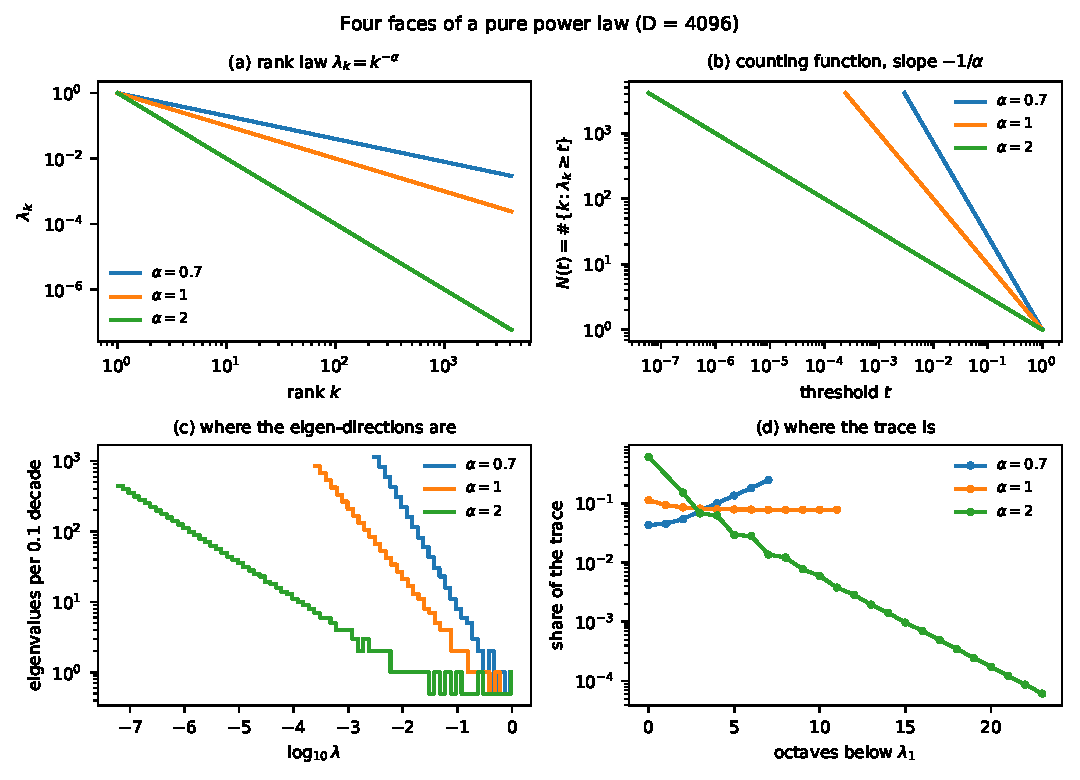
\includegraphics[width=\linewidth]{figures/faces.pdf}
\caption{Four faces of a pure power law $\lambda_k=k^{-\alpha}$, $D=4{,}096$ (synthetic). (a) The rank law.
(b) Its counting function, with slope $-1/\alpha$ (Guided proof~\ref{gp:faces}). (c) Eigenvalues per 0.1 decade:
most eigen-directions sit near the bottom (Exercise~\ref{ex:reading}). (d) Share of the trace per full octave below
$\lambda_1$: top-heavy for $\alpha=2$, flat for $\alpha=1$, bottom-heavy for $\alpha=0.7$
(Exercise~\ref{ex:octave}).}
\label{fig:faces}
\end{figure}

\begin{exercise}[Reading the exponent]\label{ex:reading}
\begin{steps}
\item Show $\lambda_{2k}/\lambda_k=2^{-\alpha}$: doubling the rank lowers the eigenvalue by $\alpha$ octaves.
\item Show that going one octave deeper ($t\mapsto t/2$) multiplies $N_A(t)$ by $2^{1/\alpha}$, up to rounding. For
  $\alpha=1$ each octave holds twice as many directions as the one above it, so most directions sit near the bottom
  (Figure~\ref{fig:faces}c).
\item Take a pure law with $\alpha=1$ and $D=4{,}096$. What percentage of the eigen-directions lies within a factor
  10 of $\lambda_1$, and what percentage within a factor 1{,}000? Which share of the trace does each group carry?
  (Answers: \NumDirWithinTen\% of the directions carry \NumTraceWithinTen{} of the trace; \NumDirWithinThousand\%
  carry \NumTraceWithinThousand.)
\end{steps}
\end{exercise}

\begin{exercise}[Transformations of a law]\label{ex:transform}
\begin{steps}
\item Show that $A\mapsto sA$ ($s>0$) changes $c$ to $sc$ and keeps $\alpha$: the exponent is scale-free.
\item Show that $A\mapsto A^p$ ($p>0$, $A$ PSD) gives exponent $\alpha p$ and scale $c^p$.
\item Precondition $A\succ0$ by a power of itself, $P=A^{-\nu}$ with $0\le\nu<1$. Show $P^{1/2}AP^{1/2}=A^{1-\nu}$,
  and give its exponent and its condition number $\lambda_1/\lambda_K$ on the window. (This is the fractional-Newton
  family of \study{noise_scale_20261021}: $\nu=0$ is the gradient step and $\nu=1$ Newton.)
\item Now precondition with a function of a \emph{different} matrix. Let $A=\diag(1,\varepsilon)$ with
  $0<\varepsilon<1$, and $P=B^{-1}$ with $B=\diag(\varepsilon,1)$: the same spectrum in the swapped frame. Compute
  the condition number of $P^{1/2}AP^{1/2}$ and compare it with that of $A$. What does this say about statements like
  (c) when $P$ has a different frame from $A$?
\end{steps}
\end{exercise}

\begin{remark}[Head law and global law]\label{rem:window}
A fit on ranks $1,\dots,K$ with $K\ll D$ describes only the top $K/D$ of $\mu_A$. The lab fits ranks 1--200 in
blocks with $D$ between 640 and 16{,}384, that is, the top 31\% down to the top 1.2\% of the eigen-directions. The
rest of $\mu_A$, where most directions live, is not covered by the fit. Section~\ref{sec:controls} works out which
quantities the fit nevertheless decides.
\end{remark}

\begin{exercise}[Broken laws]\label{ex:broken}
Let $\lambda_k=c\,k^{-\alpha_1}$ for $k\le k_b$ and $\lambda_k=c\,k_b^{-\alpha_1}(k/k_b)^{-\alpha_2}$ for
$k_b<k\le K$, so the law is continuous at the break $k_b$. Write down $N_A(t)$ on $[\lambda_K,c]$, ignoring rounding.
Show that on this range $\mu_A$ consists of two Pareto pieces, and give their tail indices.
\end{exercise}

\begin{labbox}
Early in training the lab's whitened per-tensor GGN spectra are broken. Ranks 1--16 fall roughly as $k^{-1}$ and
ranks 17--200 with $\alpha_{\text{bulk}}=1.79$--$2.10$ at steps 10--25; the break flattens by step 100. A single
law extrapolated from the top 16 then underestimates $\lambda_{17}$ by a factor 1.6--2.4
(\study{bulk_krylov_20261014}). The raw per-tensor GGN fits on ranks 1--200 go from $\alpha\approx1.8$--$2.1$ at
step 10 to $\alpha\approx0.9$--$1.1$ at steps 250--500, with $R^2\approx0.99$ (\study{spectral_rotation_20261020}).
\end{labbox}

\subsection{Kronecker products bend a law}

SOAP's eigenbasis is the Kronecker product of the eigenbases of two small factor matrices. This subsection shows that
exact power laws in the two factors do not give an exact power law in the product.

\begin{warmup}[Eigenpairs of a Kronecker product]\label{wu:kron}
For $R\in\Sym^n$ and $L\in\Sym^m$, show $(R\otimes L)(v\otimes w)=(Rv)\otimes(Lw)$. Deduce: if $Rv_j=r_jv_j$ and
$Lw_i=\ell_iw_i$, then $v_j\otimes w_i$ is an eigenvector of $R\otimes L$ with eigenvalue $r_j\ell_i$, and these $mn$
vectors are orthonormal when the $v_j$ and the $w_i$ are.
\end{warmup}

\begin{guided}[Counting a product of two laws]\label{gp:kron}
Let $\ell_i=i^{-\alpha}$ ($i\le m$) and $r_j=j^{-\alpha}$ ($j\le n$). By Warm-up~\ref{wu:kron} the eigenvalues of
$R\otimes L$ are $(ij)^{-\alpha}$. Fix $t$, set $x=t^{-1/\alpha}$, and assume $x\le\min(m,n)$.
\begin{steps}
\item Show $N(t)=\#\{(i,j):ij\le x\}=\sum_{i\le x}\floor{x/i}$.
\item Using $x/i-1<\floor{x/i}\le x/i$ and $H_n=\ln n+O(1)$, show $N(t)=x\ln x+O(x)$.
\item (Optional: Dirichlet's hyperbola trick.) Every lattice point under the hyperbola $ij\le x$ has $i\le\sqrt x$ or
  $j\le\sqrt x$. Count the two strips and subtract the square counted twice:
  $N=2\sum_{i\le\sqrt x}\floor{x/i}-\floor{\sqrt x}^2$. Deduce $N=x\ln x+(2\gamma-1)x+O(\sqrt x)$.
\item Invert. If $k=x\ln x$, show $x=k/\ln x$ and $\ln x=\ln k-\ln\ln x$. Hence $x=(k/\ln k)(1+o(1))$ and
  $\lambda_k\approx(k/\ln k)^{-\alpha}$: a power law up to a logarithm.
\item Using $k\approx x\ln x$, show that the local log--log slope is $d\ln\lambda/d\ln k=-\alpha/(1+1/\ln x)$,
  shallower than $-\alpha$.
\end{steps}
\end{guided}

\begin{compute}\label{cp:kron}
Build the $64\cdot256$ eigenvalues $(ij)^{-1}$ of the product of two pure $\alpha=1$ laws with $m=64$ and $n=256$,
sort them, and fit a straight line to $\log\lambda_k$ against $\log k$ on ranks 17--200. You should find the exponent
\NumKronSlope. Step~(e), evaluated at the geometric mean rank $k$ of the window with $x=k/\ln k$, predicts
\NumKronPred. (Reference: the end of \texttt{checks} in \texttt{make\_figures.py}.)
\end{compute}

\begin{remark}
Exact power laws in SOAP's two factors therefore appear shallower, and not exactly straight, in the product. A fitted
exponent of a Kronecker-structured matrix should not be compared one-to-one with that of an unstructured matrix.
\end{remark}

%======================================================================
\section{What the exponent decides}\label{sec:controls}
%======================================================================

Many quantities that an optimizer cares about are sums over the spectrum: the trace, the Frobenius norm,
$\tr A^{-1}$, the effective dimension under damping. For a power law each such sum is dominated either by the few
largest eigenvalues (the \emph{head}) or by the very many small ones (the \emph{tail}), and the exponent decides
which. This matters because the lab fits only the head. A fit decides head-dominated quantities and leaves
tail-dominated ones open.

\begin{reading}
Graham, Knuth \& Patashnik (1994), Section~6.3, on harmonic numbers, and Chapter~9 on asymptotics and Euler's
summation formula, the precise version of Warm-up~\ref{wu:integral}. Hastie, Tibshirani \& Friedman (2009),
Section~3.4.1, introduce the effective degrees of freedom of ridge regression, which is the effective dimension of
Section~\ref{sec:deff}.
\end{reading}

\subsection{Sums and integrals}

\begin{warmup}[Sums against integrals]\label{wu:integral}
Let $f\ge0$ be decreasing on $[m,\infty)$. Draw rectangles of width 1 under and over the graph of $f$ and show
\[\int_m^{M+1}f(x)\,dx\le\sum_{k=m}^Mf(k)\le f(m)+\int_m^Mf(x)\,dx.\]
Deduce $\ln(n+1)\le H_n\le1+\ln n$.
\end{warmup}

\begin{guided}[Power sums in three regimes]\label{gp:sums}
Let $S_s(K)=\sum_{k=1}^Kk^{-s}$.
\begin{steps}
\item ($s>1$.) Show $\sum_{k>m}k^{-s}\le m^{1-s}/(s-1)$. So the first $m$ ranks carry all but a fraction of at most
  $m^{1-s}/((s-1)\zeta(s))$ of the full sum $\zeta(s)$. For $s=2$ and $m=16$ the bound is \NumTailBoundTwo, and the
  true fraction is \NumTailTrueTwo.
\item ($s=1$.) Show that each dyadic block of ranks $\{2^j,\dots,2^{j+1}-1\}$ contributes $\ln2+O(2^{-j})$ to $H_K$:
  every block contributes about the same.
\item ($0\le s<1$.) Show $S_s(K)=K^{1-s}/(1-s)+O(1)$, and that the ranks above $K/2$ carry a fraction
  $1-2^{s-1}+o(1)$ of $S_s(K)$.
\item ($s<0$.) The terms now increase. Reverse the inequalities of Warm-up~\ref{wu:integral} and show
  $S_s(K)=K^{1-s}/(1-s)\,(1+o(1))$.
\end{steps}
\end{guided}

\begin{exercise}[Which part of a pure law decides a trace functional]\label{ex:table}
Let $\lambda_k=c\,k^{-\alpha}$ for $k=1,\dots,D$, so $\tr A^q=c^qS_{\alpha q}(D)$. Fill in the table. A functional is
decided by the head when it converges as $D\to\infty$, so that a fixed number of top ranks carries almost all of it.
Give the growth of $\tr A^{-1}$ with $D$.
\begin{center}
\begin{tabular}{lccc}
\toprule
Functional & decided by the head when & marginal at & decided by the tail when\\
\midrule
$\tr A^2=\norm{A}_\F^2$ & \hspace{6em} & \hspace{4em} & \hspace{6em}\\
$\tr A$ & & & \\
$\tr A^{1/2}$ & & & \\
$\tr A^{-1}$ & & & \\
\bottomrule
\end{tabular}
\end{center}
Which of these does a fit on ranks 1--200 decide when $\alpha\approx1$? Keep in mind that preconditioning uses
negative powers.
\end{exercise}

\begin{exercise}[At $\alpha=1$ every octave carries the same trace]\label{ex:octave}
Let $\alpha=1$.
\begin{steps}
\item Show that the eigenvalues in a full octave $[t,2t)$ carry trace $c\ln2+O(t)$.
\item Show that the top-$k$ share of the trace is $H_k/H_D\approx\ln k/\ln D$.
\item Compute it for $k=16$ and $D=640$, $4{,}096$ and $16{,}384$. (Answers: \NumShareSixForty, \NumShareFourK{} and
  \NumShareSixteenK.)
\end{steps}
\end{exercise}

\begin{labbox}
In \study{spectral_rotation_20261020} (raw per-tensor GGN on one fixed batch), the late fits (steps 250--500) give
$\alpha\approx0.9$--$1.1$ on ranks 1--200, with a slightly flatter head ($\alpha_{\text{top}}=0.65$--$0.86$) and
$\alpha_{\text{bulk}}=0.96$--$1.17$. The median top-16 share of the exact block trace over the 39 tensors is
0.35--0.45 at step 400 and 0.33--0.42 at step 500. A pure $\alpha=1$ law over all ranks gives \NumShareFourK{} for the
24 blocks with $D=4{,}096$ and \NumShareSixteenK{} for the 12 with $D=16{,}384$. The trace is the only measured
quantity that sees the whole spectrum, and it is consistent with the law extending well below rank 200. It is one
number per tensor, so this is a consistency check, not a test.

Measured spectra also leave any power law at the bottom (finite data, symmetries). In \study{noise_scale_20261021}
the smallest Ritz value of a damped whitened block $K+\delta I$ was $0.9987\,\delta$, so at least one block has
eigenvalues at numerical zero. The tail-dominated rows of Exercise~\ref{ex:table} are then set by the damping, not
by the law.
\end{labbox}

\subsection{Effective dimension under damping}\label{sec:deff}

A damped preconditioner $(A+\delta I)^{-1}$ treats directions with $\lambda\gg\delta$ as curved and directions with
$\lambda\ll\delta$ as flat. The \emph{effective dimension}
\[d_\delta(A)=\tr A(A+\delta I)^{-1}=\sum_k\frac{\lambda_k}{\lambda_k+\delta}\]
counts the curved directions softly: each contributes a number between 0 and 1. In ridge regression it is the
effective degrees of freedom.

\begin{warmup}\label{wu:deff}
For $A\in\Sym^D_+$ and $\delta>0$ show $\tfrac12N_A(\delta)\le d_\delta(A)\le N_A(\delta)+\delta^{-1}\sum_{\lambda_k<\delta}\lambda_k$.
\end{warmup}

\begin{guided}[Effective dimension of a power law]\label{gp:deff}
Let $\lambda_k=c\,k^{-\alpha}$ and $a=\delta/c$.
\begin{steps}
\item Let $f(x)=1/(1+ax^\alpha)$. Show that $d_\delta=\sum_kf(k)$, that $f$ is decreasing with $f(0)=1$, and that
  for $D=\infty$ and $\alpha>1$, $0\le\int_0^\infty f-\sum_{k\ge1}f(k)\le1$.
\item Substitute $u=a^{1/\alpha}x$ to get $\int_0^\infty f=a^{-1/\alpha}\int_0^\infty du/(1+u^\alpha)$.
\item Substitute $w=u^\alpha$ and use the Beta-function identity $\int_0^\infty w^{s-1}/(1+w)\,dw=\pi/\sin(\pi s)$
  for $0<s<1$ (a Fact; see any text on the Gamma function) to get
  $\int_0^\infty du/(1+u^\alpha)=(\pi/\alpha)/\sin(\pi/\alpha)$. Check the case $\alpha=2$ by hand.
\item Conclude $\abs[\big]{d_\delta-(c/\delta)^{1/\alpha}\,(\pi/\alpha)/\sin(\pi/\alpha)}\le1$. Damping truncates
  the law near rank $N_A(\delta)\approx(c/\delta)^{1/\alpha}$, with a factor $(\pi/\alpha)/\sin(\pi/\alpha)>1$ from
  the soft edge.
\item ($\alpha=1$, finite $D$.) Show $\abs[\big]{d_\delta-(c/\delta)\ln(1+D\delta/c)}\le1$. Here the directions below
  $\delta$ add a logarithmic factor.
\end{steps}
\end{guided}

\begin{compute}\label{cp:deff}
Check (d) for $\alpha=2$ and $\delta=10^{-6}c$, summing to rank $10^7$: \NumDdeltaExact{} against \NumDdeltaAsym.
Check (e) for $\alpha=1$, $D=4{,}096$ and $\delta=10^{-3}c$: \NumDdeltaLogExact{} against \NumDdeltaLogAsym. The
same damping keeps very different numbers of directions active for different exponents.
\end{compute}

%======================================================================
\section{The spectrum as a probability distribution}\label{sec:distribution}
%======================================================================

Suppose you know the spectrum of $A$ exactly but nothing about its frame. What should you believe about the curvature
$v^\top Av$ along a direction $v$ you care about? The natural model puts the uniform distribution on the frame. You
will show that the curvature along $v$ is then an average of the eigenvalues with random weights, that the weights
have mean $1/D$, and that the average concentrates around $\tr A/D$ at a rate set by the spread of the spectrum. This
is the precise sense in which ``the spectrum is a distribution''. The second half of the section asks what changes
once we compute: a matrix--vector product reveals the spectrum \emph{as seen from} a vector.

\begin{reading}
Meckes (2019), Chapter~1, defines Haar measure on $\Orth(D)$ and gives several constructions; Mezzadri (2007) shows
how to sample it correctly (QR of a Gaussian matrix with a sign fix). Vershynin (2018), Chapter~3, covers Gaussian
vectors, the uniform distribution on the sphere and concentration of the norm. Gelman et al.\ (2013), Appendix~A,
lists the Gamma and Dirichlet laws. Trefethen \& Bau (1997), Lectures~36--38, derive Lanczos, its link to Gauss
quadrature and conjugate gradients; Golub \& Meurant (2010) is the full treatment. Hennig, Osborne \& Kersting
(2022), the part on linear algebra, reads these methods as inference.
\end{reading}

\subsection{Spectrum known, frame unknown: the Haar model}

\begin{fact}[Haar measure]\label{fact:haar}
There is a unique probability distribution on $\Orth(D)$, the \emph{Haar} distribution, that is invariant under
multiplication: if $Q$ is Haar distributed and $R\in\Orth(D)$ is fixed, then $RQ$ and $QR$ are Haar distributed too.
\end{fact}

\begin{fact}[Direction and length of a Gaussian vector]\label{fact:gauss}
Let $g\sim\mathcal{N}(0,I_D)$. Then $g/\norm{g}$ is uniformly distributed on the unit sphere and independent of
$\norm{g}$.
\end{fact}

\begin{definition}[Haar model]\label{def:haar}
Fix $\Lambda$, draw $Q$ from the Haar distribution, and set $A=Q\Lambda Q^\top$. This models a matrix whose spectrum
is known and whose frame is not. For a fixed unit vector $v$ let $w_k=(q_k^\top v)^2$, with $q_k$ the columns of $Q$.
\end{definition}

\begin{warmup}\label{wu:haar}
\begin{steps}
\item If $g\sim\mathcal{N}(0,I_D)$ and $R\in\Orth(D)$, then $Rg\sim\mathcal{N}(0,I_D)$.
\item In the Haar model, $Q^\top v$ is uniformly distributed on the unit sphere. (Use Fact~\ref{fact:haar}.)
\item $\sum_kw_k=1$, and $\E w_k=1/D$ for every $k$.
\end{steps}
\end{warmup}

\begin{guided}[The curvature along a direction when the frame is unknown]\label{gp:haar}
Let $\psi=Q^\top v$, so that $w_k=\psi_k^2$.
\begin{steps}
\item Show $v^\top f(A)v=\sum_kf(\lambda_k)\,w_k$ for every $f$.
\item Write $\psi=g/\norm{g}$ with $g\sim\mathcal{N}(0,I_D)$ (Warm-up~\ref{wu:haar} and Fact~\ref{fact:gauss}). Use the
  independence in Fact~\ref{fact:gauss} to show $\E[g_k^4]=\E[\norm{g}^4]\,\E[w_k^2]$ and
  $\E[g_k^2g_l^2]=\E[\norm{g}^4]\,\E[w_kw_l]$.
\item Using $\E g_k^4=3$, show $\E\norm{g}^4=D(D+2)$. Deduce $\E w_k^2=3/(D(D+2))$ and, for $k\ne l$,
  $\E w_kw_l=1/(D(D+2))$.
\item Deduce $\Var w_k=2(D-1)/(D^2(D+2))$ and $\Cov(w_k,w_l)=-2/(D^2(D+2))$ for $k\ne l$.
\item\label{st:haar-var} Show $\E[v^\top f(A)v]=\int f\,d\mu_A$ and
  \[\Var[v^\top f(A)v]=\frac{2\Var_{\mu_A}(f)}{D+2},\qquad\Var_{\mu_A}(f)=\frac1D\sum_kf(\lambda_k)^2-\Bigl(\frac1D\sum_kf(\lambda_k)\Bigr)^2.\]
\item The relative standard deviation of the Rayleigh quotient $v^\top Av$ is therefore
  $\sqrt{2/(D+2)}$ times the coefficient of variation of $\mu_A$. Compute it for a pure $\alpha=1$ law with
  $D=4{,}096$. (Answer: \NumHaarRelSd.)
\end{steps}
\end{guided}

\begin{exercise}[The Dirichlet law (optional)]\label{ex:dirichlet}
\begin{steps}
\item Show that $g_k^2$ has the $\chi^2_1$ law, which is the Gamma law with shape $\frac12$ and scale 2.
\item Use the fact that independent Gamma variables with a common scale, divided by their sum, are Dirichlet
  distributed (Gelman et al.\ 2013, Appendix~A) to show $(w_1,\dots,w_D)\sim\Dir(\frac12,\dots,\frac12)$.
\item The Dirichlet$(a_1,\dots,a_D)$ moments are $\E w_k=a_k/a_0$, $\Var w_k=a_k(a_0-a_k)/(a_0^2(a_0+1))$ and
  $\Cov(w_k,w_l)=-a_ka_l/(a_0^2(a_0+1))$, with $a_0=\sum_ka_k$. Check them against Guided proof~\ref{gp:haar}(d).
\end{steps}
\end{exercise}

\begin{exercise}[The spectrum as a predictive distribution]\label{ex:mixture}
In the Haar model, draw an index $I$ with $\Pr(I=k\mid Q)=w_k$. Show that $\Pr(I=k)=1/D$, so $\lambda_I\sim\mu_A$, and
that $v^\top f(A)v=\E[f(\lambda_I)\mid Q]$.
\end{exercise}

\begin{compute}\label{cp:haar}
Check Guided proof~\ref{gp:haar}\ref{st:haar-var} for $f(\lambda)=\lambda$ by Monte Carlo, with a pure $\alpha=1$ law
and $D=256$. You need not sample $Q$: by Warm-up~\ref{wu:haar}, sample $\psi=g/\norm{g}$ directly. With
\NumHaarMCDraws{} draws, the ratio of the empirical to the predicted variance was \NumHaarMCVarRatio{} and the ratio
of the means \NumHaarMCMeanRatio. (Reference: \texttt{checks} in \texttt{make\_figures.py}.)
\end{compute}

\begin{remark}[The probabilistic-numerics reading]\label{rem:pn}
Exercise~\ref{ex:mixture} is the precise sense of ``the spectrum is a distribution''. When nothing is known about the
frame, $\mu_A$ is the prior predictive distribution of the curvature that any direction will meet. A matrix--vector
product $Av$ is an observation that changes this: it reveals part of the spectral measure seen from $v$
(Section~\ref{sec:seen}). In the language of probabilistic numerics (Hennig 2015; Wenger \& Hennig 2020; Hennig,
Osborne \& Kersting 2022), the spectrum plays the role of the prior, and computation (the products) is inference about
the frame relative to the vectors we care about. Part~III develops this.
\end{remark}

\subsection{The spectral measure seen from a vector}\label{sec:seen}

\begin{definition}\label{def:seen}
For $v\in\R^D$, the \emph{spectral measure of $A$ seen from $v$} is $\mu_{A,v}=\sum_k(u_k^\top v)^2\,\delta_{\lambda_k}$.
Its total mass is $\norm{v}^2$; its normalisation is $\nu_{A,v}=\mu_{A,v}/\norm{v}^2$.
\end{definition}

\begin{warmup}\label{wu:seen}
\begin{steps}
\item Show $\int f\,d\mu_{A,v}=v^\top f(A)v$ for every $f$, and that the total mass is $\norm{v}^2$.
\item Show $\mu_{QAQ^\top,\,Qv}=\mu_{A,v}$ for all $Q\in\Orth(D)$.
\item In the Haar model, show $\E\,\mu_{A,v}=\norm{v}^2\mu_A$ (as measures: the expected weight of each atom).
\item Let $A=\diag(\lambda_1,\dots,\lambda_D)$ with distinct entries. Compute $\nu_{A,v}$ for $v=e_1$ and for
  $v=(1,\dots,1)/\sqrt D$. The same matrix looks entirely different from different vectors.
\end{steps}
\end{warmup}

\subsection{Krylov methods read only the measure seen from the start vector}\label{sec:krylov}

\begin{fact}[Lanczos]\label{fact:lanczos}
Let $v_1$ be a unit vector, and assume that the Krylov space
\[\mathcal{K}_m=\spn\{v_1,Av_1,\dots,A^{m-1}v_1\}\]
has dimension $m$. The Lanczos iteration builds an orthonormal basis $V_m=[v_1,\dots,v_m]$ of $\mathcal{K}_m$ and a
symmetric tridiagonal $T_m=V_m^\top AV_m$ such that
\[AV_m=V_mT_m+\beta_mv_{m+1}e_m^\top,\]
with $v_{m+1}\perp\mathcal{K}_m$ a unit vector and $e_m$ the last unit vector of $\R^m$.
\end{fact}

\begin{fact}[Conjugate gradients]\label{fact:cg}
For $A\succ0$, the CG iterate $x_m$ for $Ax=b$, started at $x_0=0$, minimises $\norm{x-y}_A$ over $y\in\mathcal{K}_m(A,b)$,
where $\norm{z}_A^2=z^\top Az$.
\end{fact}

\begin{guided}[Lanczos computes a Gauss quadrature rule]\label{gp:lanczos}
\begin{steps}
\item Show that $T_m^je_1$ has non-zero entries only in its first $j+1$ positions.
\item Show by induction that $A^jv_1=V_mT_m^je_1$ for $0\le j\le m-1$. Where do you need $j\le m-1$?
\item Show $v_1^\top A^iv_1=e_1^\top T_m^ie_1$ for $0\le i\le2m-1$. (Treat even $i=2j$ and odd $i=2j+1$ separately.)
\item Write $T_m=S\Theta S^\top$ with nodes $\Theta=\diag(\theta_1,\dots,\theta_m)$ and weights $\tau_j=S_{1j}^2$.
  Show $\sum_j\tau_j\theta_j^i=\int\lambda^i\,d\nu_{A,v_1}(\lambda)$ for $0\le i\le2m-1$. The $m$-point measure
  $\sum_j\tau_j\delta_{\theta_j}$ matches $2m$ moments of $\nu_{A,v_1}$: this is the $m$-point Gauss quadrature rule
  of $\nu_{A,v_1}$.
\item Interpret: $m$ matrix--vector products reveal $2m$ moments of the spectrum seen from $v_1$. Show that $T_m$
  depends on $A$ only through these moments, so two matrices that agree on them give the same output, however
  different their frames are elsewhere.
\end{steps}
\end{guided}

\begin{guided}[The CG error is a spectral integral]\label{gp:cg}
Let $A\succ0$, $x=A^{-1}b$, and $x_m$ the CG iterate.
\begin{steps}
\item Write any $y\in\mathcal{K}_m(A,b)$ as $y=q(A)b$ with $\deg q<m$. Show $x-y=p(A)x$ with $p(\lambda)=1-\lambda q(\lambda)$,
  so $\deg p\le m$ and $p(0)=1$. Conversely, every such $p$ arises from some $q$.
\item Show $\norm{p(A)x}_A^2=b^\top A^{-1}p(A)^2b=\int p(\lambda)^2\lambda^{-1}\,d\mu_{A,b}(\lambda)$.
\item Conclude
  \[\norm{x-x_m}_A^2=\min\Bigl\{\int p(\lambda)^2\lambda^{-1}\,d\mu_{A,b}(\lambda):\deg p\le m,\ p(0)=1\Bigr\}.\]
  Two matrices with different frames but the same measure seen from $b$ produce the same CG errors at every step.
\item If $\mu_{A,b}$ has only $r$ atoms, show that CG is exact after $r$ steps.
\end{steps}
\end{guided}

The \texttt{weights} returned by the lab's \path{noise_scale_20261021/scripts/lanczos.py} are exactly the $\tau_j$ of
Guided proof~\ref{gp:lanczos}(d).

\subsection{One step on a quadratic, and the value of curvature}

\begin{exercise}[The best step along a direction]\label{ex:step}
Let $A\succ0$, $g\in\R^D$ and $q(x)=\frac12x^\top Ax-g^\top x$. For $f>0$ on the spectrum, show that the best decrease
along $x=\eta f(A)g$, $\eta\in\R$, is
\[\max_\eta\bigl[q(0)-q(\eta f(A)g)\bigr]=\frac{\bigl(\int f\,d\mu_{A,g}\bigr)^2}{2\int\lambda f(\lambda)^2\,d\mu_{A,g}(\lambda)}.\]
\end{exercise}

\begin{guided}[Kantorovich's inequality]\label{gp:kantorovich}
Let $\nu$ be a probability measure on $[m,M]$ with $0<m<M$, and $\kappa=M/m$.
\begin{steps}
\item Use Exercise~\ref{ex:step} to show that the ratio of the best decreases of Newton ($f=1/\lambda$) and of a tuned
  gradient step ($f=1$) is $\E_\nu[\lambda]\,\E_\nu[\lambda^{-1}]$ with $\nu=\nu_{A,g}$.
\item Show $\E_\nu[\lambda]\,\E_\nu[\lambda^{-1}]\ge1$ (Cauchy--Schwarz or Jensen).
\item For $\lambda\in[m,M]$, show $(\lambda-m)(M-\lambda)\ge0$ and deduce $\lambda+mM/\lambda\le m+M$.
\item Integrate against $\nu$ and use $2\sqrt{xy}\le x+y$ to show
  $\E_\nu[\lambda]\,\E_\nu[\lambda^{-1}]\le(m+M)^2/(4mM)=(\kappa+1)^2/(4\kappa)$.
\end{steps}
\end{guided}

\begin{exercise}[Uniform weights on a power law]\label{ex:kantpower}
Let $\lambda_k=c/k$, $k=1,\dots,D$, and $\nu=\mu_A$ (a gradient with equal weight on every eigen-direction). Show
$\E_\mu[\lambda]\,\E_\mu[\lambda^{-1}]=H_D(D+1)/(2D)\approx\frac12\ln D$. Compute it for $D=4{,}096$ and $16{,}384$
(answers: \NumKantFourK{} and \NumKantSixteenK) and compare with Kantorovich's worst case for $\kappa=D=4{,}096$,
which is \NumKantWorstFourK. What decides the value of curvature: the spectrum or the weights?
\end{exercise}

\begin{remark}[Two measures decide a step]\label{rem:twomeasures}
With batch noise of covariance $\Sigma$, the denominator in Exercise~\ref{ex:step} gains the term
$(1/B-1/N)\int\lambda f^2\,d\mu_{A,\Sigma}$, where $\mu_{A,\Sigma}=\sum_k(u_k^\top\Sigma u_k)\,\delta_{\lambda_k}$
(\texttt{batch\_noise.md}, T1). For one step, all that matters about $A$ is the pair $(\mu_{A,\bar g},\mu_{A,\Sigma})$:
how the signal and the noise are spread over the spectrum. The frame enters only through these weights. Two questions
follow for training. Does the gradient's measure $\nu_{A,\bar g}$ stay stationary while the frame rotates, that is,
does the gradient co-rotate with the frame? And how do it and $\mu_{A,\Sigma}$ change during training? The forms
$z^\top A^qz$, $q\in[-1,1]$, measured in \study{noise_scale_20261021} are moments of exactly these measures.
\end{remark}

%======================================================================
\section{Perturbation: what a power law implies about the frame}\label{sec:perturbation}
%======================================================================

Curvature matrices in training are never known exactly. A different batch, a later step or a cheaper estimator gives
$B=A+E$ instead of $A$. This section asks how far eigenvalues and eigenvectors move. The answer is asymmetric.
Eigenvalues move by at most the size of $E$, whatever the spectrum. Eigenvectors move by the size of $E$ divided by
the gap to the neighbouring eigenvalues. A power law has gaps that shrink like $\lambda_k/k$, so going down the
spectrum, eigenvectors are lost much earlier than eigenvalues.

\begin{reading}
Bhatia (1997) is the best single source: Chapter~III (variational principles, Weyl), Chapter~VI (Hoffman--Wielandt),
Chapter~VII (Davis--Kahan $\sin\Theta$ theorems) and Chapter~X (perturbation of matrix functions). Horn \& Johnson
(2013), Sections~4.2--4.3, cover Courant--Fischer, Weyl and Schur's majorization. Yu, Wang \& Samworth (2015) is a
short paper written for statisticians that states the Davis--Kahan version we use; Davis \& Kahan (1970) is the
original, and Stewart \& Sun (1990) the standard monograph. Kato (1976), Chapter~II, treats analytic perturbation in
finite dimensions.
\end{reading}

\begin{warmup}[Everything in a $2\times2$ matrix]\label{wu:twobytwo}
Let $A=\diag(a,b)$ with gap $g=a-b>0$, and $E=\delta\begin{psmallmatrix}0&1\\1&0\end{psmallmatrix}$ with $\delta>0$.
\begin{steps}
\item Show that the eigenvalues of $A+E$ are $\frac{a+b}2\pm\sqrt{g^2/4+\delta^2}$. Each moves by
  $\sqrt{g^2/4+\delta^2}-g/2$, which lies in $[0,\delta]$ and is about $\delta^2/g$ when $\delta\ll g$.
\item Show that the top eigenvector of $A+E$ is $(\cos\theta,\sin\theta)$ with $\tan2\theta=2\delta/g$.
\item For $a=1$, $b=0.99$ and $\delta=0.01$, compute both. (Answers: the eigenvalues move by \NumTwoShift, the
  eigenvector rotates by \NumTwoAngle$^\circ$.)
\item Let $g\to0$ with $\delta$ fixed. What happens to $\theta$, and what does that say about who decides the
  eigenvector, $A$ or $E$?
\end{steps}
\end{warmup}

\subsection{Eigenvalues are stable}

\begin{guided}[Courant--Fischer]\label{gp:courant}
Show $\lambda_k(A)=\max_{\dim S=k}\ \min_{v\in S,\,\norm{v}=1}v^\top Av$, the maximum over subspaces $S$ of dimension $k$.
\begin{steps}
\item For $S=\spn(u_1,\dots,u_k)$, show that the inner minimum is $\lambda_k$.
\item For any $S$ of dimension $k$, show $S\cap\spn(u_k,\dots,u_D)\ne\{0\}$ by counting dimensions.
\item For a unit $v$ in that intersection show $v^\top Av\le\lambda_k$, and conclude.
\end{steps}
\end{guided}

\begin{guided}[Weyl's inequality]\label{gp:weyl}
Let $B=A+E$. Show $\abs{\lambda_k(B)-\lambda_k(A)}\le\norm{E}_\op$ for every $k$.
\begin{steps}
\item Show $v^\top Bv\le v^\top Av+\norm{E}_\op$ for every unit $v$.
\item Insert this into Courant--Fischer to get $\lambda_k(B)\le\lambda_k(A)+\norm{E}_\op$. Swap the roles of $A$ and
  $B$.
\end{steps}
\end{guided}

\begin{fact}[Birkhoff--von Neumann]\label{fact:birkhoff}
A matrix with non-negative entries whose rows and columns all sum to 1 is \emph{doubly stochastic}. Every doubly
stochastic matrix is a convex combination of permutation matrices. Hence a linear function on the doubly stochastic
matrices attains its maximum at a permutation matrix. (Bhatia 1997, Chapter~II.)
\end{fact}

\begin{exercise}[Rearrangement inequality]\label{ex:rearrange}
Let $a_1\ge\dots\ge a_D$ and $b_1\ge\dots\ge b_D$. Show $\sum_ia_ib_{\pi(i)}\le\sum_ia_ib_i$ for every permutation
$\pi$. Start with two indices: if $i<j$ but $\pi(i)>\pi(j)$, swapping the two values does not decrease the sum.
\end{exercise}

\begin{guided}[Hoffman--Wielandt]\label{gp:hw}
Let $A=U_A\diag(a)U_A^\top$ and $B=U_B\diag(b)U_B^\top$ with sorted spectra $a$ and $b$. Show
$\sum_k(a_k-b_k)^2\le\norm{A-B}_\F^2$.
\begin{steps}
\item Show $\norm{A-B}_\F^2=\sum_ia_i^2+\sum_jb_j^2-2\tr(AB)$.
\item With $W=U_A^\top U_B$, show $\tr(AB)=\sum_{i,j}a_ib_jW_{ij}^2$.
\item Show that the matrix $P=(W_{ij}^2)$ is doubly stochastic.
\item Use Fact~\ref{fact:birkhoff} and Exercise~\ref{ex:rearrange} to show $\tr(AB)\le\sum_ia_ib_i$, and conclude.
\end{steps}
\end{guided}

\begin{exercise}[Spectra are close as distributions]\label{ex:wasserstein}
For two probability measures on $\R$ that put mass $1/D$ on each of $D$ points, an optimal coupling for the
Wasserstein-2 distance can be taken to be a permutation (Fact~\ref{fact:birkhoff} again; Santambrogio 2015,
Chapter~2). Use Exercise~\ref{ex:rearrange} to show that the sorted coupling is optimal, and deduce
$W_2(\mu_A,\mu_B)\le\norm{A-B}_\F/\sqrt D$.
\end{exercise}

\subsection{Eigenvectors are only as stable as their gaps}

\begin{guided}[A one-vector $\sin\theta$ theorem]\label{gp:sintheta}
Let $B=A+E$, fix $k$, and let $g_k=\min_{j\ne k}\abs{\lambda_j(A)-\lambda_k(A)}>0$ be the gap of $\lambda_k(A)$ to the
rest of the spectrum. Let $u=u_k(A)$, $v=u_k(B)$, $\mu=\lambda_k(B)$, and $P=I-uu^\top$. Then
$\sin\angle(u,v)=\norm{Pv}$.
\begin{steps}
\item Show $(A-\mu I)v=-Ev$.
\item Show that $P$ commutes with $A$, so $P(A-\mu I)v=(A-\mu I)Pv$.
\item $Pv$ lies in $\spn\{u_j:j\ne k\}$. Show that on this span $\norm{(A-\mu I)z}\ge\min_{j\ne k}\abs{\lambda_j-\mu}\,\norm{z}$,
  and use Weyl to get $\min_{j\ne k}\abs{\lambda_j-\mu}\ge g_k-\norm{E}_\op$.
\item Combine (a)--(c) with $\norm{PEv}\le\norm{E}_\op$ to get $\sin\angle(u,v)\le\norm{E}_\op/(g_k-\norm{E}_\op)$
  when $\norm{E}_\op<g_k$.
\item Conclude $\sin\angle(u,v)\le2\norm{E}_\op/g_k$ in all cases.
\end{steps}
\end{guided}

\begin{remark}[The subspace version]\label{rem:dk}
The same idea, with $P$ replaced by the projector onto the complement of the top-$k$ eigenspace, gives the version of
Yu, Wang \& Samworth (2015) for the top-$k$ subspaces: $\norm{\sin\Theta}_\F\le2\min(\sqrt k\norm{E}_\op,\norm{E}_\F)/(\lambda_k-\lambda_{k+1})$,
where $\sin\Theta$ collects the sines of the principal angles between the two subspaces. Only the gap at the cut
enters, not the gaps inside the subspace.
\end{remark}

\begin{exercise}[Gaps of a power law]\label{ex:gaps}
Let $\lambda_k=c\,k^{-\alpha}$.
\begin{steps}
\item Show that $h(x)=1-(1+x)^{-\alpha}$ is concave with $h(0)=0$, and deduce $xh'(x)\le h(x)\le xh'(0)$ for $x\ge0$.
\item With $x=1/k$, deduce $\frac{\alpha}{k}(1+\frac1k)^{-\alpha-1}\le(\lambda_k-\lambda_{k+1})/\lambda_k\le\frac{\alpha}{k}$.
\item Show that consecutive gaps decrease, so that for $2\le k<D$ the gap $g_k$ of Guided proof~\ref{gp:sintheta} is
  $\lambda_k-\lambda_{k+1}$ (and $g_1=\lambda_1-\lambda_2$).
\end{steps}
\end{exercise}

\begin{guided}[Two resolution limits]\label{gp:resolution}
Let $A$ follow a pure law $(c,\alpha)$, let $\norm{B-A}_\op\le\eta$, and let $s\in(0,1]$.
\begin{steps}
\item Show $\abs{\lambda_k(B)-\lambda_k(A)}\le s\lambda_k(A)$ for every $k\le K_{\text{val}}:=(sc/\eta)^{1/\alpha}$.
\item Use Exercise~\ref{ex:gaps} and $1+1/k\le2$ to show $g_k\ge\alpha c\,k^{-\alpha-1}2^{-\alpha-1}$ for $k<D$.
\item Use Guided proof~\ref{gp:sintheta} to show $\sin\angle(u_k(A),u_k(B))\le s$ for every $k<D$ with
  $k\le K_{\text{vec}}:=\bigl(s\alpha c/(2^{\alpha+2}\eta)\bigr)^{1/(\alpha+1)}$.
\item Show $K_{\text{vec}}/K_{\text{val}}\to0$ as $\eta\to0$: for small perturbations far more eigenvalues than
  eigenvectors are resolved. Eigenvalues are resolved to depth $\propto\eta^{-1/\alpha}$, eigenvectors only to
  $\propto\eta^{-1/(\alpha+1)}$.
\end{steps}
\end{guided}

\begin{exercise}[Numbers for the guarantees]\label{ex:resnumbers}
Take $\alpha=1$, $c=1$, $s=1/2$ and $\eta=\NumSimEtaScaled\times10^{-4}$, the operator norm of the Gaussian
perturbation used in Figure~\ref{fig:resolution}. Compute $K_{\text{val}}$ and $K_{\text{vec}}$. (Answers:
\NumKvalWeyl{} and \NumKvecWorst.) The simulation in Figure~\ref{fig:resolution} resolves eigenvalues to rank
\NumKvalSim{} and eigenvectors to rank \NumKvecSim. Which guarantee is more pessimistic, and why might a worst-case
bound be pessimistic for a random $E$?
\end{exercise}

\subsection{Typical perturbations: first-order theory}

Worst-case bounds assume that $E$ is aligned as badly as possible with the frame of $A$. A random $E$ is not. First-order
perturbation theory gives the typical sizes with explicit constants.

\begin{guided}[First-order perturbation theory]\label{gp:firstorder}
Let $A$ have distinct eigenvalues and $A(\varepsilon)=A+\varepsilon E$. Accept (Kato 1976, Chapter~II) that
$\lambda_k(\varepsilon)$ and unit eigenvectors $u_k(\varepsilon)$ can be chosen differentiable near $\varepsilon=0$.
Write $'$ for $d/d\varepsilon$ at $\varepsilon=0$.
\begin{steps}
\item Differentiate $A(\varepsilon)u_k(\varepsilon)=\lambda_k(\varepsilon)u_k(\varepsilon)$ to get
  $Eu_k+Au_k'=\lambda_k'u_k+\lambda_ku_k'$.
\item Multiply by $u_k^\top$ to get $\lambda_k'=u_k^\top Eu_k$.
\item Multiply by $u_j^\top$, $j\ne k$, to get $u_j^\top u_k'=u_j^\top Eu_k/(\lambda_k-\lambda_j)$.
\item Differentiate $u_k^\top u_k=1$ to get $u_k^\top u_k'=0$. Conclude
  \[u_k'=\sum_{j\ne k}\frac{u_j^\top Eu_k}{\lambda_k-\lambda_j}\,u_j,\qquad
  \sin\angle(u_k(0),u_k(\varepsilon))=\varepsilon\norm{u_k'}+O(\varepsilon^2).\]
  Compare with Guided proof~\ref{gp:orbit}\ref{st:orbit-entries}.
\end{steps}
\end{guided}

\begin{exercise}[Typical sizes for Gaussian noise]\label{ex:typical}
Let $E=\varepsilon G$, where $G$ is symmetric with independent centred Gaussian entries, of variance 1 off the
diagonal and 2 on it. Then $Q^\top GQ$ has the law of $G$ for every fixed $Q\in\Orth(D)$ (accept this), and
$\norm{E}_\op\approx2\varepsilon\sqrt D$.
\begin{steps}
\item Show that $u_j^\top Gu_k$, $j\ne k$, are independent $\mathcal{N}(0,1)$ and $u_k^\top Gu_k\sim\mathcal{N}(0,2)$.
  Deduce that, to first order, $\E\sin^2\angle(u_k(A),u_k(B))\approx\varepsilon^2\sum_{j\ne k}(\lambda_k-\lambda_j)^{-2}$,
  and that an eigenvalue moves by about $\sqrt2\varepsilon$.
\item For a pure law, split the sum, and use $g_k\approx\alpha c\,k^{-\alpha-1}$. Show that the neighbouring ranks
  contribute $\sum_{m\ne0}(mg_k)^{-2}\approx2\zeta(2)k^{2\alpha+2}/(\alpha^2c^2)$, and that the many much smaller
  eigenvalues contribute about $Dk^{2\alpha}/c^2$.
\item Show that the neighbours dominate once $k\gtrsim\alpha\sqrt{D/(2\zeta(2))}$. For $\alpha=1$ and
  $D=\NumSimDim$ this is about \NumNeighbourRank.
\item Show that the typical eigenvector resolution limit, where the sine reaches $s$, is
  $k_{\text{vec}}\approx\bigl(s\alpha c/(\sqrt{2\zeta(2)}\,\varepsilon)\bigr)^{1/(\alpha+1)}$. For $\alpha=1$, $c=1$,
  $s=1/2$ and $\varepsilon=10^{-5}$ this is \NumKvecPred.
\end{steps}
\end{exercise}

\begin{compute}\label{cp:resolution}
Reproduce Figure~\ref{fig:resolution}(a) and~(b). Take $\lambda_k=1/k$ with $D=\NumSimDim$, $E=\varepsilon(Z+Z^\top)/\sqrt2$
with $Z$ a standard Gaussian matrix and $\varepsilon=10^{-5}$, and compute the eigen-decomposition of
$\diag(\lambda)+E$. Why may you take $A$ diagonal? Over three draws (medians) you should find relative eigenvalue
errors below $\NumRelValTopScaled\times10^{-3}$ in the top 100 ranks, reaching 0.5 only at rank \NumKvalSim, and
eigenvector sines reaching 0.5 at rank \NumKvecSim{} (predicted \NumKvecPred). (Reference: \texttt{figure\_resolution}
in \texttt{make\_figures.py}.)
\end{compute}

\begin{figure}[t]
\centering
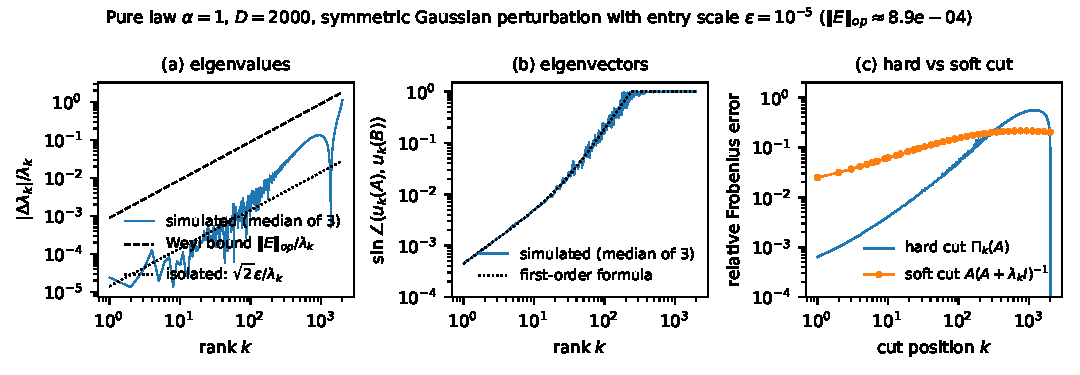
\includegraphics[width=\linewidth]{figures/resolution.pdf}
\caption{Resolution limits (synthetic). A pure $\alpha=1$ law, $D=\NumSimDim$, perturbed by a symmetric Gaussian
matrix with entry scale $\varepsilon=10^{-5}$; medians of three draws. (a) Relative eigenvalue errors, with Weyl's
bound and the isolated-eigenvalue estimate $\sqrt2\varepsilon/\lambda_k$. (b) Eigenvector angles, with the
first-order formula of Exercise~\ref{ex:typical}. (c) Relative Frobenius error of the top-$k$ projector (hard cut)
and of the soft cut $A(A+\lambda_kI)^{-1}$ at the same place (Remark~\ref{rem:cut}).}
\label{fig:resolution}
\end{figure}

\subsection{Functions of the matrix: hard and soft cuts}

A preconditioner is a function of an estimated matrix. Which functions survive a perturbation? Smooth ones do, in the
Frobenius norm, whatever the eigenvectors did. A hard cut onto the top $k$ eigenvectors survives only as well as the
gap at the cut.

\begin{guided}[Lipschitz spectral functions are as stable as the matrix]\label{gp:lipschitz}
Let $f$ be $L$-Lipschitz on an interval that contains the spectra of $A=U_A\diag(a)U_A^\top$ and
$B=U_B\diag(b)U_B^\top$. Show $\norm{f(A)-f(B)}_\F\le L\norm{A-B}_\F$.
\begin{steps}
\item With $W=U_A^\top U_B$, show that $U_A^\top(A-B)U_B$ has entries $(a_i-b_j)W_{ij}$.
\item Show that $U_A^\top(f(A)-f(B))U_B$ has entries $(f(a_i)-f(b_j))W_{ij}$.
\item Use that the Frobenius norm is unchanged by orthogonal factors, and compare the two matrices entry by entry.
\end{steps}
In the operator norm the same statement fails with constant $L$; see Bhatia (1997), Chapter~X.
\end{guided}

\begin{exercise}[Damping sets the stability of a fractional step]\label{ex:fractional}
Show that $f(\lambda)=(\lambda+\delta)^{-\nu}$, $\nu>0$, is $\nu\delta^{-\nu-1}$-Lipschitz on $[0,\infty)$. Deduce
$\norm{(A+\delta I)^{-\nu}-(B+\delta I)^{-\nu}}_\F\le\nu\delta^{-\nu-1}\norm{A-B}_\F$ for PSD $A$ and $B$, whatever
the eigenvectors did.
\end{exercise}

\begin{exercise}[Distance between projectors]\label{ex:projector}
Let $P$ and $P'$ be orthogonal projectors of rank $k$, and let $\cos^2\theta_1,\dots,\cos^2\theta_k$ be the squared
singular values of $V^\top V'$ for orthonormal bases $V$ and $V'$ of their ranges. Show
$\norm{P-P'}_\F^2=2(k-\norm{PP'}_\F^2)=2\sum_i\sin^2\theta_i=2\norm{\sin\Theta}_\F^2$. With Remark~\ref{rem:dk}, the
top-$k$ projector $\Pi_k$ satisfies
$\norm{\Pi_k(A)-\Pi_k(B)}_\F\le2\sqrt2\min(\sqrt k\norm{E}_\op,\norm{E}_\F)/(\lambda_k-\lambda_{k+1})$: no bound of
the kind in Guided proof~\ref{gp:lipschitz} holds, because the indicator of $\{\lambda\ge\lambda_k\}$ is not Lipschitz.
\end{exercise}

\begin{remark}[A cut or a smooth function?]\label{rem:cut}
The two bounds have different strengths, and Figure~\ref{fig:resolution}c shows both effects. A hard cut where the
gap is large is far more stable than a smooth ``soft cut'' $A(A+\lambda_kI)^{-1}$ at the same place: at $k=16$ the
relative errors are \NumHardSixteen{} (hard) and \NumSoftSixteen{} (soft). The smooth function acts on every direction
and pays for the perturbation everywhere; its error is controlled by $\norm{E}_\F$, which grows like $\varepsilon D$.
Deep in the spectrum, where gaps are tiny, the order reverses: at $k\approx1{,}000$ the errors are \NumHardThousand{}
(hard) and \NumSoftThousand{} (soft). The curves cross at $k\approx\NumCrossCut$, about twice the eigenvector
resolution limit. (Soft-cut values are on a grid of cut positions; the ones quoted are at \NumSoftCuts.)

The design rule this suggests is not ``never store a frame'' but: cut only where the frame is resolved, and use
smooth functions of the current matrix beyond that. PARSEC-L's brake $I-\sum_{k\le r}\frac{\kappa_k}{1+\kappa_k}w_kw_k^\top$
with $\kappa_k=c_{\mathrm b}\eta\lambda_k$ is exactly the soft function $\lambda/(\lambda+1/(c_{\mathrm b}\eta))$
applied inside a hard top-$r$ cut. Its fully smooth version is $(I+c_{\mathrm b}\eta K)^{-1}$, which needs no
eigenvectors.
\end{remark}

\subsection{Stale frame, fresh diagonal}

SOAP and EKFAC keep a frame $U$ computed from an earlier matrix and refresh only a diagonal in that frame. What is
the best diagonal for a given frame, and what does a stale frame cost?

\begin{warmup}[Pinching]\label{wu:pinching}
For a frame $U$ and $A\in\Sym^D$ let
\[\mathcal{P}_U(A)=U\diag(u_1^\top Au_1,\dots,u_D^\top Au_D)\,U^\top.\]
Among the matrices $UMU^\top$ with $M$ diagonal, show that $\mathcal{P}_U(A)$ is the closest to $A$ in Frobenius
norm, and that $\norm{A-\mathcal{P}_U(A)}_\F^2=\sum_{i\ne j}(u_i^\top Au_j)^2$. Show also $\tr\mathcal{P}_U(A)=\tr A$.
\end{warmup}

\begin{guided}[Ky Fan's principle and Schur's majorization]\label{gp:kyfan}
\begin{steps}
\item Let $x_1,\dots,x_k$ be orthonormal and $X=[x_1,\dots,x_k]$. Show $\sum_ix_i^\top Ax_i=\sum_j\lambda_jc_j$ with
  $c_j=\norm{X^\top u_j}^2$.
\item Show $0\le c_j\le1$ and $\sum_jc_j=k$.
\item Show that $\sum_j\lambda_jc_j$ under these constraints is at most $\lambda_1+\dots+\lambda_k$.
\item Apply this to the $k$ columns of $U$ with the largest Rayleigh quotients $u_i^\top Au_i$. Conclude that the
  Rayleigh quotients are \emph{majorised} by the eigenvalues: for every $k$ the sum of the $k$ largest is at most
  $\lambda_1+\dots+\lambda_k$, with equality for $k=D$.
\item Deduce $\max_iu_i^\top Au_i\le\lambda_1(A)$ and $\min_iu_i^\top Au_i\ge\lambda_D(A)$: a stale frame flattens
  the effective spectrum.
\end{steps}
\end{guided}

\begin{remark}[The bridge to SOAP]\label{rem:soap}
This is the structure of EKFAC and SOAP: a frame refreshed rarely and a diagonal refreshed every step.
Warm-up~\ref{wu:pinching} is the Frobenius-optimality argument that George et al.\ (2018) give for EKFAC's diagonal,
and Eschenhagen et al.\ (2025) analyse Shampoo and SOAP in the same Frobenius terms. Guided proof~\ref{gp:kyfan} adds
what a stale frame costs spectrally: the effective spectrum is flattened, with the top lowered and the bottom raised,
the more so the further the frame has drifted. That is the direction of the shrinkage that rotationally invariant
estimators from random-matrix statistics apply when eigenvectors are unreliable (Bun, Bouchaud \& Potters 2017). Two
cautions for Part~III: SOAP's diagonal is an exponential average of squared rotated gradients, a second moment of the
gradient rather than the GGN; and it enters through a square root.
\end{remark}

\begin{labbox}
Late in training, the 10-step capture of a cached top-$k$ subspace rises with $k$: 0.78--0.84 at $k=1$ and 0.87--0.91
at $k=200$ (\study{spectral_rotation_20261020}). The study read this as mixing within nearly tied groups, which is
what Guided proof~\ref{gp:resolution} and Exercise~\ref{ex:typical} predict for a power law. But the late head is
flatter ($\alpha_{\text{top}}=0.65$--$0.86$), so the relative gap below the top eigenvalue is
$1-2^{-\alpha_{\text{top}}}\approx0.36$--$0.45$, which is not small. Losing 16--22\% of the top direction's curvature
in 10 steps therefore means the 10-step change is not small compared with the top gap. Part~II has to allow changes
that are large at the top, not only mixing among near-ties. Rotation also exceeds batch noise: at fixed weights
another batch's top-16 subspace captures 0.93--0.999.
\end{labbox}

%======================================================================
\section{Towards Part II}\label{sec:next}
%======================================================================

Part~I treated one matrix. Part~II lets it move. The first guided proof below is the equation of motion of spectrum
and frame; you have already met it twice.

\begin{guided}[How spectrum and frame move]\label{gp:motion}
Let $A(t)=U(t)\Lambda(t)U(t)^\top$ be differentiable with distinct eigenvalues and differentiable $U(t)\in\Orth(D)$.
\begin{steps}
\item Show that $W=U^\top U'$ is skew-symmetric.
\item Show $U^\top A'U=\Lambda'+W\Lambda-\Lambda W$.
\item Deduce $\lambda_k'=u_k^\top A'u_k$ and, for $i\ne j$, $W_{ij}=u_i^\top A'u_j/(\lambda_j-\lambda_i)$. Check that
  this is Guided proof~\ref{gp:firstorder} with $E=A'$.
\item Interpret: ``stable spectrum, rotating frame'' means that $A'$ is nearly off-diagonal in the current eigenbasis.
  The rotation rate of a pair of eigenvectors is the off-diagonal entry of $A'$ divided by their gap.
\end{steps}
\end{guided}

\begin{exercise}[Two fingerprints]\label{ex:dyson}
\begin{steps}
\item (Isotropic noise.) Suppose that over a short time $h$ the matrix changes by $\Delta A=\sigma\sqrt h\,G$, with $G$
  as in Exercise~\ref{ex:typical} and independent of the past. To first order, show that the rotation of the pair
  $(i,j)$ over that time, $hW_{ij}$, has variance $\sigma^2h/(\lambda_i-\lambda_j)^2$, while $\lambda_k$ changes with
  variance $2\sigma^2h$, independent of the gaps. Pairs with small gaps rotate fastest. (With the second-order terms
  this becomes Dyson Brownian motion; Tao 2012 and Allez \& Bouchaud 2012.)
\item (Frame diffusion.) Suppose instead $U'=UW$ with $W$ a random skew-symmetric matrix whose law does not depend
  on $\Lambda$, and $\Lambda'=0$. How large are the off-diagonal entries of $U^\top A'U$ now, as a function of the
  gaps?
\item Which measurement on saved spectra and eigenvectors would tell the two pictures apart?
\end{steps}
\end{exercise}

\paragraph{The plan for Part~II.}
\begin{enumerate}[(1),itemsep=1pt]
\item Three stochastic pictures with different fingerprints: isotropic matrix noise (rotation rate $\propto$
  gap$^{-2}$), frame diffusion (rate independent of the gaps) and deterministic drift (ballistic, hence predictable).
  Their fingerprints are capture against lag (linear or quadratic onset), rotation against gap, and replicas forked
  with different data orders.
\item Structure: the change of a GGN under a weight step is not isotropic. What is its structure?
\item Data: \study{spectral_rotation_20261020} saved spectra and captures; replays (10--12 minutes per trajectory)
  give eigenvectors. \study{noise_scale_20261021}'s forms give moments of the gradient's and the noise's spectral
  measures at 36 states without new compute.
\end{enumerate}

\subsection*{What is known (searches of 23 October 2026)}

References marked $^*$ were checked online on 23 October 2026, at least at the level of the abstract; the others are
cited from memory.
\begin{itemize}[itemsep=1pt]
\item \textbf{EKFAC} (George et al.\ 2018$^*$): the eigenbasis is recomputed rarely and the diagonal tracked every
  step, justified by cost and a Frobenius argument (Warm-up~\ref{wu:pinching}). No model of how the eigenbasis moves.
\item \textbf{SOAP} (Vyas et al.\ 2024$^*$): Adam in Shampoo's eigenbasis. The refresh interval is studied
  empirically; there is no model of eigenbasis drift against eigenvalue drift and no theory of the optimal interval.
\item \textbf{Purifying Shampoo} (Eschenhagen et al.\ 2025$^*$): decouples eigenvalue and eigenbasis updates and
  proposes an adaptive refresh criterion that controls the current approximation error. It does not forecast the
  error from a model of the frame's motion.
\item \textbf{Power-law Hessian spectra}: Xie et al.\ (2022$^*$) and Tang et al.\ (2025$^*$). \textbf{Eigenvector
  dynamics}: Gur-Ari, Roberts \& Dyer (2018); Marjankowska, Modugno \& Barucca (2026$^*$).
\item \textbf{Random-matrix statistics}: rotationally invariant estimators (Ledoit \& P\'ech\'e 2011; Bun et al.\
  2016$^*$; Bun, Bouchaud \& Potters 2017$^*$); eigenvector dynamics of exponentially weighted covariance matrices,
  the estimator family of SOAP's statistics (Allez \& Bouchaud 2012).
\item \textbf{Probabilistic numerics}: Hennig \& Kiefel (2013); Hennig (2015); de Roos \& Hennig (2019$^*$); Wenger \&
  Hennig (2020); Tatzel et al.\ (2025$^*$).
\end{itemize}
As far as these searches show, no published work treats the spectral law as (nearly) stationary and the frame as a
latent process, and derives SOAP's refresh schedule, averaging windows or treatment of momentum from such a model.
Searches can miss work; this should be re-checked before any claim of novelty. The compact note,
\texttt{spectral\_frame.pdf}, Section~7, has the full list with comments.

\subsection*{Questions for us}
\begin{question}
Which matrix should the theory treat first: the GGN, which we measured, or SOAP's own statistic, Kronecker factors of
gradient second moments (Guided proof~\ref{gp:kron})?
\end{question}
\begin{question}
Is a scale-free law the right null hypothesis, given that the trace grows 1.3--1.6$\times$ during the learning-rate
decay while the shape does not (\study{spectral_rotation_20261020})?
\end{question}
\begin{question}
Which prior on the frame: uniform (Haar), or concentrated around SOAP's current basis (a matrix Bingham or
von~Mises--Fisher law)?
\end{question}
\begin{question}
Which first measurement: rotation against gap from replays (Exercise~\ref{ex:dyson}), or the gradient's spectral
measure, which the forms saved by \study{noise_scale_20261021} give for free?
\end{question}

%======================================================================
\appendix
% Appendix A of workbook.tex: hints, in the order of the items. Input by workbook.tex after \appendix.
\section{Hints}\label{app:hints}

Hints are short on purpose. If a hint gives too much away, read only its first sentence.

\newcommand{\hint}[2]{\item[#1~\ref{#2}.]}
\newenvironment{hintlist}{\begin{description}[leftmargin=0pt,itemsep=3pt,font=\normalfont\bfseries]}{\end{description}}

\subsection*{Section~\ref{sec:frame}}
\begin{hintlist}
\hint{Warm-up}{wu:spectrum} (a) $\tr(XY)=\tr(YX)$, and $\norm{A}_\F^2=\tr(A^\top A)$. (b), (c) Write $v=Uz$; then
$\norm{v}=\norm{z}$ and $v^\top Av=\sum_k\lambda_kz_k^2$. (d) For ``only if'', test $v=u_D$.
\hint{Warm-up}{wu:orthogonal} Compute $u^\top Aw$ in two ways.
\hint{Exercise}{ex:fwelldef} (a) $A^i=U\Lambda^iU^\top$. (b) $p(A)$ is computed from $A$ alone. (c) Powers of $A$
commute with $A$. For the inverse, multiply $(A+\delta I)$ by $U\diag(1/(\lambda_k+\delta))U^\top$.
\hint{Warm-up}{wu:rotate} $(QAQ^\top)(Qu_k)=QAu_k$. For $f$, use the polynomial $p$ of Exercise~\ref{ex:fwelldef}.
\hint{Guided proof}{gp:orbit} (a) Product rule at $t=0$; $(e^{tW})^\top=e^{tW^\top}$. (b) Which entries of a
skew-symmetric matrix are free? (c) Product rule, with $Q(0)=I$ and $Q'(0)^\top=-W$. (d) $(W\Lambda)_{ij}=W_{ij}\lambda_j$.
(e) For the image: given $S$, try $W_{ij}=S_{ij}/(\lambda_j-\lambda_i)$. (f) $(\lambda_j-\lambda_i)W_{ij}=0$ allows
$W_{ij}\ne0$ exactly when $\lambda_i=\lambda_j$. (g) $Q\Lambda=\Lambda Q$; compare entries as in (d).
\hint{Exercise}{ex:invariant} Choose $Q=U^\top$.
\hint{Warm-up}{wu:examples} Test with $Q=U^\top$, where $U$ is a frame of a $2\times2$ matrix with non-zero
off-diagonal entries, or with a permutation matrix.
\hint{Guided proof}{gp:equivariant} (a) $R_k^2=I$. (b) Check $R_kAR_k$ on the basis $u_1,\dots,u_D$. (c) Take $Q=R_k$
in the definition. (d) $R_kG(A)u_k=G(A)R_ku_k$. (e) Interpolate as in Exercise~\ref{ex:fwelldef}.
\hint{Exercise}{ex:krylovequiv} $(QAQ^\top)^i=QA^iQ^\top$, so the numbers $b^\top A^ib$ do not change.

\end{hintlist}

\subsection*{Section~\ref{sec:faces}}
\begin{hintlist}
\hint{Warm-up}{wu:small} $N_A$ is a step function that jumps at $t=3$, $1$ and $0$; decide which value it takes at
each jump point.
\hint{Exercise}{ex:quantile} (a) The spectrum is sorted. (b) What is the set $\{t:N_A(t)\ge k\}$? (c) Divide by $D$.
\hint{Guided proof}{gp:faces} (a) Sorted spectrum. (b) $t\ge\lambda_K=cK^{-\alpha}$. (c) Count integers. (d)
Differentiate the tail and change its sign. (e) $t=ce^{-v}$. (f) Evaluate $N_A$ at $t=ck^{-\alpha}$ and just above it.
\hint{Exercise}{ex:reading} (c) $\lambda_k\ge\lambda_1/10$ if and only if $k\le10$; the trace share is $H_{10}/H_{4096}$.
\hint{Exercise}{ex:transform} (b), (c) Functions of $A$ keep its frame. (d) $P^{1/2}=\diag(\varepsilon^{-1/2},1)$.
\hint{Exercise}{ex:broken} On the lower piece, solve $c\,k_b^{-\alpha_1}(k/k_b)^{-\alpha_2}\ge t$ for $k$.
\hint{Warm-up}{wu:kron} Mixed-product rule $(X\otimes Y)(Z\otimes T)=(XZ)\otimes(YT)$, and
$(v\otimes w)^\top(v'\otimes w')=(v^\top v')(w^\top w')$.
\hint{Guided proof}{gp:kron} (a) For fixed $i$, which $j$ are allowed? Why is $j\le n$ automatic? (b)
$\sum_{i\le x}x/i=xH_{\floor x}$. (c) Use $H_s=\ln s+\gamma+O(1/s)$ with $s=\floor{\sqrt x}$, and $s^2=x+O(\sqrt x)$.
(d) Take logarithms. (e) Compute $d\ln k/d\ln x$ for $k=x\ln x$.

\end{hintlist}

\subsection*{Section~\ref{sec:controls}}
\begin{hintlist}
\hint{Warm-up}{wu:integral} For $k\ge m$: $f(k+1)\le\int_k^{k+1}f\le f(k)$. Sum.
\hint{Guided proof}{gp:sums} (a) Compare the tail with $\int_m^\infty x^{-s}dx$. (b) The warm-up with $f(x)=1/x$ on one
block. (c) The warm-up with $m=1$; for the share, compute $S_s(K)-S_s(K/2)$. (d) For increasing $f$:
$\int_{k-1}^kf\le f(k)\le\int_k^{k+1}f$.
\hint{Exercise}{ex:table} $\tr A^q$ is a power sum with $s=\alpha q$; Guided proof~\ref{gp:sums} has one case for each
column. For $q=-1$, $s=-\alpha<0$.
\hint{Exercise}{ex:octave} (a) The eigenvalues in $[t,2t)$ have ranks $c/(2t)<k\le c/t$. (b) Divide two harmonic
numbers.
\hint{Warm-up}{wu:deff} Split the sum at $\delta$: $\lambda/(\lambda+\delta)\ge\frac12$ if and only if $\lambda\ge\delta$,
and $\lambda/(\lambda+\delta)\le\lambda/\delta$.
\hint{Guided proof}{gp:deff} (a) $\lambda_k/(\lambda_k+\delta)=1/(1+\delta/\lambda_k)$. For the comparison, use
$f(k)\le\int_{k-1}^kf$ and $\int_k^{k+1}f\le f(k)$, plus $\int_0^1f\le1$. (b) $dx=a^{-1/\alpha}du$. (c)
$du=\frac1\alpha w^{1/\alpha-1}dw$, so $s=1/\alpha$; for $\alpha=2$ the integral is an arctangent. (e) The same
comparison on $[0,D]$.
\hint{Compute}{cp:deff} $10^7$ float64 values take 80\,MB; summing them in one numpy call is fine.

\end{hintlist}

\subsection*{Section~\ref{sec:distribution}}
\begin{hintlist}
\hint{Warm-up}{wu:haar} (a) A linear map of a Gaussian vector is Gaussian; compute the covariance. (b)
$R(Q^\top v)=(QR^\top)^\top v$. The uniform law is the only rotation-invariant law on the sphere. (c) Take $R$ a
permutation matrix in (b).
\hint{Guided proof}{gp:haar} (a) $f(A)=Qf(\Lambda)Q^\top$. (b) $g_k=\norm{g}\psi_k$. (c) Expand
$\norm{g}^4=(\sum_kg_k^2)^2$. (d) $\Var X=\E X^2-(\E X)^2$. (e) $\Var\sum_kf_kw_k=\sum_{k,l}f_kf_l\Cov(w_k,w_l)$;
separate $k=l$ from $k\ne l$. (f) Use $\sum_kk^{-2}\approx\zeta(2)$, or compute numerically.
\hint{Exercise}{ex:dirichlet} (a) Change variables $y=g^2$ in the Gaussian density. (c) $a_k=\frac12$ and $a_0=D/2$.
\hint{Exercise}{ex:mixture} Average $\Pr(I=k\mid Q)=w_k$ over $Q$.
\hint{Compute}{cp:haar} Draw $g$ in batches of, say, 20{,}000 rows to keep memory small. Use the population variance
of the eigenvalues for $\Var_{\mu_A}$.
\hint{Warm-up}{wu:seen} (a) $f(A)=\sum_kf(\lambda_k)u_ku_k^\top$. (b) The eigenvectors of $QAQ^\top$ are $Qu_k$. (c)
Warm-up~\ref{wu:haar}(c). (d) Here $u_k=e_k$.
\hint{Guided proof}{gp:lanczos} (a) Induction: multiplying by a tridiagonal matrix extends the support by one
position. (b) $AV_mT_m^je_1=V_mT_m^{j+1}e_1+\beta_mv_{m+1}(e_m^\top T_m^je_1)$; when is the last factor zero? (c)
$v_1^\top A^{2j}v_1=\norm{A^jv_1}^2$ and $v_1^\top A^{2j+1}v_1=(A^jv_1)^\top A(A^jv_1)$, with $V_m^\top AV_m=T_m$. (d)
$e_1^\top T_m^ie_1=e_1^\top S\Theta^iS^\top e_1$.
\hint{Guided proof}{gp:cg} (a) $b=Ax$. (b) Functions of $A$ commute. (d) Choose $p(\lambda)=\prod_j(1-\lambda/\lambda_j)$
over the atoms.
\hint{Exercise}{ex:step} The objective is a quadratic in $\eta$; then use Warm-up~\ref{wu:seen}(a).
\hint{Guided proof}{gp:kantorovich} (a) Insert $f=1/\lambda$ and $f=1$ into Exercise~\ref{ex:step} and divide. (b)
$1=(\E[\lambda^{1/2}\lambda^{-1/2}])^2$. (c) Expand and divide by $\lambda>0$. (d) Apply $2\sqrt{xy}\le x+y$ to
$x=\E_\nu\lambda$ and $y=mM\,\E_\nu\lambda^{-1}$.
\hint{Exercise}{ex:kantpower} $\E_\mu\lambda=\frac1D\sum_kc/k$ and $\E_\mu\lambda^{-1}=\frac1D\sum_kk/c$.

\end{hintlist}

\subsection*{Section~\ref{sec:perturbation}}
\begin{hintlist}
\hint{Warm-up}{wu:twobytwo} (a) Characteristic polynomial. (b) Write the two rows of the eigenvector equation,
multiply them by $\sin\theta$ and $\cos\theta$, and subtract. (d) $\tan2\theta\to\infty$.
\hint{Guided proof}{gp:courant} (a) $v=\sum_{i\le k}z_iu_i$. (b) $k+(D-k+1)>D$. (c) $v=\sum_{i\ge k}z_iu_i$.
\hint{Guided proof}{gp:weyl} (a) $v^\top Ev\le\norm{E}_\op$ for unit $v$. (b) Apply (a) to every $v$ in every $S$.
\hint{Exercise}{ex:rearrange} Swapping an inversion changes the sum by $(a_i-a_j)(b_{\pi(j)}-b_{\pi(i)})$.
\hint{Guided proof}{gp:hw} (b) $\tr(AB)=\tr(\diag(a)\,W\diag(b)\,W^\top)$. (c) Rows and columns of an orthogonal matrix
are unit vectors. (d) $\tr(AB)$ is linear in $P$.
\hint{Exercise}{ex:wasserstein} For a permutation coupling the cost is $\frac1D\sum_i(a_i-b_{\pi(i)})^2$; expand the
square.
\hint{Guided proof}{gp:sintheta} (b) $Auu^\top=\lambda_kuu^\top=uu^\top A$. (c) Expand $z$ in the eigenvectors $u_j$,
$j\ne k$. (d) $\norm{(A-\mu I)Pv}=\norm{PEv}$. (e) Consider $\norm{E}_\op\le g_k/2$ and $\norm{E}_\op>g_k/2$
separately.
\hint{Exercise}{ex:gaps} (a) Concave functions lie below their tangents. (b) $(\lambda_k-\lambda_{k+1})/\lambda_k=h(1/k)$.
(c) $x\mapsto cx^{-\alpha}$ is convex.
\hint{Guided proof}{gp:resolution} (a) Weyl. (b) $(1+1/k)^{-\alpha-1}\ge2^{-\alpha-1}$. (c) Solve $2\eta/g_k\le s$ for
$k$. (d) The ratio is a power of $\eta$.
\hint{Exercise}{ex:resnumbers} With $\alpha=c=1$: $K_{\text{val}}=s/\eta$ and $K_{\text{vec}}=(s/(8\eta))^{1/2}$. On
which pair of directions would a worst-case $E$ put its size?
\hint{Guided proof}{gp:firstorder} (b) $u_k^\top A=\lambda_ku_k^\top$, so two terms cancel. (c) $u_j^\top u_k=0$. (d)
Expand $u_k'$ in the basis $u_1,\dots,u_D$.
\hint{Exercise}{ex:typical} (a) Take $Q=U$. (b) For $\abs{m}\ll k$, $\lambda_k-\lambda_{k+m}\approx-mg_k$, and
$\sum_{m\ne0}m^{-2}=2\zeta(2)$; for $j\gg k$, $(\lambda_k-\lambda_j)^{-2}\approx\lambda_k^{-2}$. (d) Set
$\varepsilon\sqrt{2\zeta(2)}k^{\alpha+1}/(\alpha c)=s$.
\hint{Compute}{cp:resolution} $(Z+Z^\top)/\sqrt2$ has off-diagonal variance 1 and diagonal variance 2.
The function \texttt{eigh} in \texttt{numpy.linalg} returns ascending eigenvalues; reverse them. The sine of the $k$-th angle is
$\sqrt{1-(e_k^\top v_k)^2}$.
\hint{Guided proof}{gp:lipschitz} (a) $U_A^\top A=\diag(a)U_A^\top$ and $BU_B=U_B\diag(b)$. (c) Entrywise,
$\abs{f(a_i)-f(b_j)}\le L\abs{a_i-b_j}$.
\hint{Exercise}{ex:fractional} Bound the derivative.
\hint{Exercise}{ex:projector} $\norm{P-P'}_\F^2=\tr P+\tr P'-2\tr(PP')$ and $\tr(PP')=\norm{V^\top V'}_\F^2$.
\hint{Warm-up}{wu:pinching} $\norm{A-UMU^\top}_\F=\norm{U^\top AU-M}_\F$.
\hint{Guided proof}{gp:kyfan} (a) Expand $x_i$ in the eigenvectors. (b) Bessel's inequality. (c) Moving weight to a
larger $\lambda_j$ never decreases the sum. (e) $k=1$, and the case $k=D-1$ subtracted from the trace.

\end{hintlist}

\subsection*{Section~\ref{sec:next}}
\begin{hintlist}
\hint{Guided proof}{gp:motion} (a) Differentiate $U^\top U=I$. (b) Differentiate $A=U\Lambda U^\top$ and multiply by
$U^\top$ on the left and $U$ on the right. (c) Guided proof~\ref{gp:orbit}\ref{st:orbit-entries}.
\hint{Exercise}{ex:dyson} (a) Exercise~\ref{ex:typical}(a) with $\Delta A$ in place of $E$. (b) Read off
$(U^\top A'U)_{ij}=(\lambda_j-\lambda_i)W_{ij}$. (c) Plot a measured rotation against the gap.
\end{hintlist}

\ifdefined\withsolutions
% Appendix B of workbook.tex: solutions. Input only when \withsolutions is defined (workbook_solutions.tex).
\clearpage
\section{Solutions}\label{app:solutions}

\newcommand{\sol}[2]{\paragraph{#1~\ref{#2}.}}

%----------------------------------------------------------------------
\subsection*{Section~\ref{sec:frame}}

\sol{Warm-up}{wu:spectrum}
(a) $\tr A=\tr(U\Lambda U^\top)=\tr(\Lambda U^\top U)=\tr\Lambda$. Likewise $\norm{A}_\F^2=\tr(A^\top A)$, which
equals $\tr(U\Lambda^2U^\top)=\sum_k\lambda_k^2$.
\newline (b) For $v=Uz$,
\[\norm{Av}=\norm{U\Lambda z}=\norm{\Lambda z}\le\max_k\abs{\lambda_k}\,\norm{z}=\max_k\abs{\lambda_k}\,\norm{v},\]
with equality for $z=e_k$ at the largest $\abs{\lambda_k}$.
\newline (c) $v^\top Av=z^\top\Lambda z=\sum_k\lambda_kz_k^2$ lies between $\lambda_D\sum_kz_k^2$ and $\lambda_1\sum_kz_k^2$,
and $\sum_kz_k^2=\norm{v}^2$; equality at $z=e_D$ and $z=e_1$.
\newline (d) If $\lambda_D\ge0$, (c) gives $v^\top Av\ge0$. If $A$ is PSD, $\lambda_D=u_D^\top Au_D\ge0$.

\sol{Warm-up}{wu:orthogonal}
$u^\top Aw=\mu\,u^\top w$ and, by symmetry, $u^\top Aw=(Au)^\top w=\lambda\,u^\top w$. So $(\lambda-\mu)u^\top w=0$.

\sol{Exercise}{ex:fwelldef}
(a) $A^i=U\Lambda^iU^\top$ by induction, so $p(A)=Up(\Lambda)U^\top=U\diag(p(\lambda_k))U^\top=U\diag(f(\lambda_k))U^\top$.
\newline (b) $p$ depends only on $f$ and the values $\lambda_k$, and $p(A)$ is computed from $A$ without any frame.
\newline (c) $p(A)A=Ap(A)$ because powers of $A$ commute. $A^2$ is $f(A)$ for $f(\lambda)=\lambda^2$. For $\delta>-\lambda_D$,
$(A+\delta I)\,U\diag(1/(\lambda_k+\delta))U^\top=U\diag((\lambda_k+\delta)/(\lambda_k+\delta))U^\top=I$, so the inverse is
$f(A)$ with $f(\lambda)=1/(\lambda+\delta)$. For PSD $A$, $U\diag(\lambda_k^{1/2})U^\top$ is PSD and squares to $A$;
$(A+\delta I)^{-\nu}$ is defined as $f(A)$ with $f(\lambda)=(\lambda+\delta)^{-\nu}$, which agrees with the inverse
for $\nu=1$.

\sol{Warm-up}{wu:rotate}
$\norm{Qv}^2=v^\top Q^\top Qv=\norm{v}^2$. $(QAQ^\top)(Qu_k)=QAu_k=\lambda_kQu_k$, and the $Qu_k$ are orthonormal, so
$QAQ^\top=(QU)\Lambda(QU)^\top$ has spectrum $\sigma(A)$ and frame $QU$. Hence
$f(QAQ^\top)=QUf(\Lambda)U^\top Q^\top=Qf(A)Q^\top$.

\sol{Guided proof}{gp:orbit}
(a) $\frac{d}{dt}(Q^\top Q)=Q'^\top Q+Q^\top Q'=0$; at $t=0$ this is $W^\top+W=0$. For skew $W$,
$(e^{tW})^\top=e^{tW^\top}=e^{-tW}$, and $e^{-tW}e^{tW}=I$ because $tW$ and $-tW$ commute.
\newline (b) $W_{ii}=-W_{ii}$ forces a zero diagonal, and the entries below the diagonal are fixed by those above, which are
free: $D(D-1)/2$ numbers.
\newline (c) $A'=Q'\Lambda Q^\top+Q\Lambda Q'^\top$, which at $t=0$ is $W\Lambda+\Lambda W^\top=W\Lambda-\Lambda W$.
\newline (d) $(W\Lambda)_{ij}=W_{ij}\lambda_j$ and $(\Lambda W)_{ij}=\lambda_iW_{ij}$.
\newline (e) If $(\lambda_j-\lambda_i)W_{ij}=0$ for all $i\ne j$ and the $\lambda$'s are distinct, every off-diagonal $W_{ij}$
vanishes; the diagonal vanishes anyway, so $W=0$. The image is symmetric, since
$(W\Lambda-\Lambda W)^\top=-\Lambda W+W\Lambda$, and has zero diagonal by (d). Conversely, for symmetric $S$ with zero
diagonal, $W_{ij}=S_{ij}/(\lambda_j-\lambda_i)$ ($i\ne j$) is skew-symmetric and maps to $S$. So the orbit has
$D(D-1)/2$ independent directions at $\Lambda$, the diagonal matrices add $D$ more, and together they span $\Sym^D$,
of dimension $D(D+1)/2$.
\newline (f) $W_{ij}(\lambda_j-\lambda_i)=0$ for all $i,j$ allows $W_{ij}\ne0$ exactly when $\lambda_i=\lambda_j$, that is,
inside the diagonal blocks of equal values. Inside a block of size $m_j$, $W$ is an arbitrary skew-symmetric
$m_j\times m_j$ matrix, so the kernel has dimension $\sum_jm_j(m_j-1)/2$ and the image $D(D-1)/2-\sum_jm_j(m_j-1)/2$.
\newline (g) $Q\Lambda Q^\top=\Lambda$ means $Q\Lambda=\Lambda Q$, that is, $Q_{ij}(\lambda_j-\lambda_i)=0$, so $Q$ is
diagonal; a diagonal orthogonal matrix satisfies $Q_{ii}^2=1$. If $U\Lambda U^\top=V\Lambda V^\top$, then
$Q=U^\top V$ satisfies $Q\Lambda Q^\top=\Lambda$, so $V=UQ$: the columns agree up to sign.

\sol{Exercise}{ex:invariant}
If $F$ is invariant, $F(A)=F(U^\top AU)=F(\diag\sigma(A))$. Conversely, if $F(A)=\varphi(\sigma(A))$, then
$F(QAQ^\top)=\varphi(\sigma(QAQ^\top))=\varphi(\sigma(A))$ by Warm-up~\ref{wu:rotate}.

\sol{Warm-up}{wu:examples}
(a) $\tr A$, $\det A$, $\lambda_1(A)$ and $\norm{A}_\F$ are functions of the spectrum, hence invariant. $A_{11}$ and
$v^\top Av$ are not: for $A=\diag(1,0)$ and $Q$ the swap of the two coordinates, $(QAQ^\top)_{11}=0\ne1$.
\newline (b) $A^2$, $(A+\delta I)^{-1}$ and $\Pi_k(A)$ are equivariant, by Warm-up~\ref{wu:rotate}: each is a function of $A$
(for $\Pi_k$, the indicator of $[\lambda_k,\infty)$). $\Diag(A)$ is not: for
$A=\begin{psmallmatrix}0&1\\1&0\end{psmallmatrix}$, $\Diag(A)=0$, but with $Q=U^\top$ ($U$ a frame of $A$),
$QAQ^\top=\diag(1,-1)$ has $\Diag(QAQ^\top)=\diag(1,-1)\ne Q\,0\,Q^\top$. $A+B_0$ is equivariant only if
$QB_0Q^\top=B_0$ for all $Q$, which forces $B_0=cI$.

\sol{Guided proof}{gp:equivariant}
(a) $R_k^\top=R_k$ and $R_k^2=I-4u_ku_k^\top+4u_k(u_k^\top u_k)u_k^\top=I$. $R_ku_k=u_k-2u_k=-u_k$ and $R_ku_j=u_j$
for $j\ne k$. Since the $u_j$ form a basis, the $-1$ eigenspace is $\spn(u_k)$.
\newline (b) $R_kAR_ku_j=R_kA(\pm u_j)=\pm\lambda_jR_ku_j=\lambda_ju_j=Au_j$ for every $j$.
\newline (c) Equivariance with $Q=R_k$: $G(A)=G(R_kAR_k^\top)=R_kG(A)R_k$.
\newline (d) By (c), $G(A)u_k=R_kG(A)R_ku_k=-R_kG(A)u_k$, so $R_k(G(A)u_k)=-G(A)u_k$ and $G(A)u_k\in\spn(u_k)$.
\newline (e) $G(A)U=U\diag(\varphi)$, so $G(A)=U\diag(\varphi)U^\top$, which commutes with $A=U\Lambda U^\top$. For distinct
eigenvalues choose $p$ with $p(\lambda_k)=\varphi_k$; then $p(A)=U\diag(\varphi)U^\top$.

\sol{Exercise}{ex:krylovequiv}
$(Qb)^\top(QAQ^\top)^i(Qb)=b^\top Q^\top QA^iQ^\top Qb=b^\top A^ib$, so $p_{QAQ^\top,Qb}=p_{A,b}=:p$ and
$F(QAQ^\top,Qb)=p(QAQ^\top)Qb=Qp(A)Q^\top Qb=QF(A,b)$. With a stored frame,
$x'=U_{\mathrm{old}}\diag(\varphi)U_{\mathrm{old}}^\top Qb$ is in general not $Qx$: the result depends on how $A$ and $b$
sit relative to $U_{\mathrm{old}}$. The stored frame is a third argument, and only rotating it along ($QU_{\mathrm{old}}$)
restores equivariance.

%----------------------------------------------------------------------
\subsection*{Section~\ref{sec:faces}}

\sol{Warm-up}{wu:small}
$\mu_A=\frac14\delta_3+\frac12\delta_1+\frac14\delta_0$. $N_A(t)=4$ for $t\le0$, $3$ for $0<t\le1$, $1$ for $1<t\le3$
and $0$ for $t>3$; it jumps down just after each eigenvalue. The rank function is $(3,1,1,0)$. At $t=1$, $N_A=3$:
for $k=2,3$ both $\lambda_k=1\ge1$ and $3\ge k$ hold; for $k=4$ both fail.

\sol{Exercise}{ex:quantile}
(a) If $\lambda_k\ge t$, then $\lambda_1,\dots,\lambda_k\ge t$, so $N_A(t)\ge k$. If at least $k$ eigenvalues are
$\ge t$, the $k$ largest are, and in particular $\lambda_k$.
\newline (b) By (a), $\{t:N_A(t)\ge k\}=(-\infty,\lambda_k]$, whose maximum is $\lambda_k$.
\newline (c) $\mu_A([t,\infty))\ge k/D$ if and only if $N_A(t)\ge k$, so $Q_A(k/D)=\max\{t:N_A(t)\ge k\}=\lambda_k$.

\sol{Guided proof}{gp:faces}
(a) For $k>K$: $\lambda_k\le\lambda_{K+1}<\lambda_K\le t$.
\newline (b) $ck^{-\alpha}\ge t\iff k^\alpha\le c/t\iff k\le(c/t)^{1/\alpha}$, and $t\ge\lambda_K=cK^{-\alpha}$ gives
$(c/t)^{1/\alpha}\le K$.
\newline (c) $N_A(t)$ counts the integers $1\le k\le(c/t)^{1/\alpha}$, all of which are $\le K$.
\newline (d) Divide by $D$. Without the floor, $\mu_A([t,\infty))=(c/t)^{1/\alpha}/D=\frac KD(t/\lambda_K)^{-1/\alpha}$ on
$[\lambda_K,c]$: $K/D$ times the tail of a Pareto law with index $1/\alpha$ and minimum $\lambda_K$. The density is
$-\frac{d}{dt}\bigl[(c/t)^{1/\alpha}/D\bigr]=\frac1\alpha c^{1/\alpha}t^{-1/\alpha-1}/D$.
\newline (e) With $t=ce^{-v}$, $(c/t)^{1/\alpha}=e^{v/\alpha}$, and $t\ge\lambda_K\iff v\le\alpha\ln K$.
\newline (f) Let $k\le K$ and $t_k=ck^{-\alpha}\ge cK^{-\alpha}$. Then $N_A(t_k)=k$, so $\lambda_k\ge t_k$ by
Exercise~\ref{ex:quantile}\ref{st:quantile-a}. For $t>t_k$, $(c/t)^{1/\alpha}<k$, so $N_A(t)<k$ and $\lambda_k<t$.
Hence $\lambda_k=t_k$.

\sol{Exercise}{ex:reading}
(a) $c(2k)^{-\alpha}/(ck^{-\alpha})=2^{-\alpha}$.
\newline (b) $(c/(t/2))^{1/\alpha}=2^{1/\alpha}(c/t)^{1/\alpha}$.
\newline (c) $\lambda_k=c/k\ge c/10$ if and only if $k\le10$: $10/4096=\NumDirWithinTen\%$ of the directions, carrying
$H_{10}/H_{4096}=\NumTraceWithinTen$ of the trace. Within a factor 1{,}000: $k\le1000$, that is \NumDirWithinThousand\%
of the directions, carrying $H_{1000}/H_{4096}=\NumTraceWithinThousand$. The bottom three quarters of the directions
carry the remaining sixth of the trace.

\sol{Exercise}{ex:transform}
(a) $s\lambda_k=(sc)k^{-\alpha}$.
\newline (b) $A^p$ has eigenvalues $\lambda_k^p=c^pk^{-\alpha p}$, in the same frame and the same order.
\newline (c) $P^{1/2}=A^{-\nu/2}$, and all three matrices are functions of $A$ with the frame $U$, so
$P^{1/2}AP^{1/2}=U\Lambda^{-\nu/2}\Lambda\Lambda^{-\nu/2}U^\top=A^{1-\nu}$. Exponent $\alpha(1-\nu)$, scale $c^{1-\nu}$,
condition number $K^{\alpha(1-\nu)}$ on the window.
\newline (d) $P^{1/2}=\diag(\varepsilon^{-1/2},1)$ and $P^{1/2}AP^{1/2}=\diag(1/\varepsilon,\varepsilon)$, with condition number
$\varepsilon^{-2}$ against $\varepsilon^{-1}$ for $A$: the wrong frame squares the condition number instead of
reducing it. Statements like (c) use that $P$ and $A$ share a frame. Otherwise the result depends on the relative
frame, not on the two spectra alone.

\sol{Exercise}{ex:broken}
For $t\ge\lambda_{k_b}=ck_b^{-\alpha_1}$, $N_A(t)=(c/t)^{1/\alpha_1}$ as in Guided proof~\ref{gp:faces}. For
$\lambda_K\le t<\lambda_{k_b}$, $\lambda_{k_b}(k/k_b)^{-\alpha_2}\ge t\iff k\le k_b(\lambda_{k_b}/t)^{1/\alpha_2}$, so
$N_A(t)=k_b(\lambda_{k_b}/t)^{1/\alpha_2}$. Both formulas give $k_b$ at $t=\lambda_{k_b}$. So $\mu_A$ has a Pareto
piece with tail index $1/\alpha_1$ on $[\lambda_{k_b},c]$ and one with tail index $1/\alpha_2$ on
$[\lambda_K,\lambda_{k_b})$.

\sol{Warm-up}{wu:kron}
The mixed-product rule gives $(R\otimes L)(v\otimes w)=(Rv)\otimes(Lw)$, and for eigenvectors this is
$(r_jv_j)\otimes(\ell_iw_i)=r_j\ell_i\,(v_j\otimes w_i)$. Also
$(v_j\otimes w_i)^\top(v_{j'}\otimes w_{i'})=(v_j^\top v_{j'})(w_i^\top w_{i'})$, which is 1 if $(j,i)=(j',i')$ and 0
otherwise: $mn$ orthonormal vectors in $\R^{mn}$, a full frame.

\sol{Guided proof}{gp:kron}
(a) $(ij)^{-\alpha}\ge t\iff ij\le x$. For each $i\le x$ the allowed $j$ are $1,\dots,\floor{x/i}$, all $\le n$
because $x\le n$; and $i\le x\le m$.
\newline (b) $\sum_{i\le x}(x/i-1)<N\le\sum_{i\le x}x/i$, that is, $xH_{\floor x}-\floor x<N\le xH_{\floor x}$, and
$H_{\floor x}=\ln x+O(1)$.
\newline (c) If $i>\sqrt x$ and $j>\sqrt x$, then $ij>x$; so every counted point has $i\le s$ or $j\le s$, with
$s=\floor{\sqrt x}$. The strip $i\le s$ holds $\sum_{i\le s}\floor{x/i}$ points, the strip $j\le s$ as many, and both
strips share the $s^2$ points with $i,j\le s$ (all counted, since $ij\le s^2\le x$). Then
$\sum_{i\le s}\floor{x/i}=xH_s+O(s)=x(\tfrac12\ln x+\gamma)+O(\sqrt x)$, using $\ln s=\frac12\ln x+O(1/\sqrt x)$, and
$s^2=x+O(\sqrt x)$. So $N=x\ln x+2\gamma x-x+O(\sqrt x)$.
\newline (d) $x\ln x=k$ gives $x=k/\ln x$, and taking logarithms $\ln x=\ln k-\ln\ln x=\ln k\,(1+o(1))$. So
$x=(k/\ln k)(1+o(1))$ and $\lambda_k=x^{-\alpha}\approx(k/\ln k)^{-\alpha}$.
\newline (e) $\ln k=\ln x+\ln\ln x$, so $d\ln k/d\ln x=1+1/\ln x$; with $\ln\lambda=-\alpha\ln x$,
$d\ln\lambda/d\ln k=-\alpha/(1+1/\ln x)$.

\sol{Compute}{cp:kron}
\begin{verbatim}
lam = np.sort(np.outer(1/np.arange(1, 65), 1/np.arange(1, 257)).ravel())[::-1]
k = np.arange(17, 201)
slope = np.polyfit(np.log(k), np.log(lam[k-1]), 1)[0]          # about -0.77
km = np.exp(np.mean(np.log(k))); x = km/np.log(km)
predicted = 1/(1+1/np.log(x))                                  # about 0.75
\end{verbatim}

%----------------------------------------------------------------------
\subsection*{Section~\ref{sec:controls}}

\sol{Warm-up}{wu:integral}
For $x\in[k,k+1]$, $f(k+1)\le f(x)\le f(k)$; integrate: $f(k+1)\le\int_k^{k+1}f\le f(k)$. Summing the right
inequality over $k=m,\dots,M$ gives the lower bound. Summing the left one over $k=m,\dots,M-1$ gives
$\sum_{k=m+1}^Mf(k)\le\int_m^Mf$; add $f(m)$. With $f(x)=1/x$, $m=1$ and $M=n$: $\ln(n+1)\le H_n\le1+\ln n$.

\sol{Guided proof}{gp:sums}
(a) $\sum_{k>m}k^{-s}\le\int_m^\infty x^{-s}dx=m^{1-s}/(s-1)$; divide by $\zeta(s)$. For $s=2$, $m=16$:
$(1/16)/\zeta(2)=\NumTailBoundTwo$, against the true \NumTailTrueTwo.
\newline (b) With $f(x)=1/x$ on the block, $\ln2=\int_{2^j}^{2^{j+1}}dx/x\le\sum_{k=2^j}^{2^{j+1}-1}1/k\le2^{-j}+\int_{2^j}^{2^{j+1}-1}dx/x\le2^{-j}+\ln2$.
\newline (c) With $m=1$, $M=K$: $((K+1)^{1-s}-1)/(1-s)\le S_s(K)\le1+(K^{1-s}-1)/(1-s)$, and
$0\le(K+1)^{1-s}-K^{1-s}\le(1-s)K^{-s}\le1-s$ by the mean value theorem; so both bounds are $K^{1-s}/(1-s)+O(1)$. Then
$S_s(K)-S_s(K/2)=(K^{1-s}-(K/2)^{1-s})/(1-s)+O(1)$, and dividing by $S_s(K)$, with $K^{1-s}\to\infty$, gives
$1-2^{s-1}+o(1)$.
\newline (d) For increasing $f(x)=x^{-s}=x^{\abs s}$: $\int_{k-1}^kf\le f(k)\le\int_k^{k+1}f$, so
$K^{1-s}/(1-s)=\int_0^Kf\le S_s(K)\le\int_1^{K+1}f\le(K+1)^{1-s}/(1-s)$, and both bounds are
$K^{1-s}/(1-s)\,(1+o(1))$.

\sol{Exercise}{ex:table}
With $s=\alpha q$: head-dominated if $\alpha q>1$ (case (a)); marginal at $\alpha q=1$, with equal contributions per
octave (case (b)); tail-dominated if $\alpha q<1$, where the ranks above $D/2$ keep a fixed share (cases (c) and (d)).
\begin{center}
\begin{tabular}{lccc}
\toprule
Functional & head when & marginal at & tail when\\
\midrule
$\tr A^2$ & $\alpha>1/2$ & $\alpha=1/2$ & $\alpha<1/2$\\
$\tr A$ & $\alpha>1$ & $\alpha=1$ & $\alpha<1$\\
$\tr A^{1/2}$ & $\alpha>2$ & $\alpha=2$ & $\alpha<2$\\
$\tr A^{-1}$ & never & --- & always; $\approx c^{-1}D^{1+\alpha}/(1+\alpha)$\\
\bottomrule
\end{tabular}
\end{center}
At $\alpha\approx1$ a fit on ranks 1--200 decides $\tr A^2$ (by (a), ranks beyond 200 carry at most about $0.3\%$ of
it), decides $\tr A$ only up to the logarithm of the unseen ranks, and decides neither $\tr A^{1/2}$ nor any negative
power.

\sol{Exercise}{ex:octave}
(a) $c/k\in[t,2t)\iff c/(2t)<k\le c/t$: one dyadic block of ranks, up to rounding at its ends, starting near
$a=c/(2t)$. By Guided proof~\ref{gp:sums}(b) its sum is $c(\ln2+O(1/a))=c\ln2+O(t)$.
\newline (b) $\sum_{j\le k}(c/j)/\sum_{j\le D}(c/j)=H_k/H_D$, and $H_n\approx\ln n$.
\newline (c) $H_{16}=3.381$, $H_{640}=7.039$, $H_{4096}=8.895$ and $H_{16384}=10.281$ give \NumShareSixForty, \NumShareFourK{}
and \NumShareSixteenK.

\sol{Warm-up}{wu:deff}
Terms with $\lambda_k\ge\delta$ lie in $[\frac12,1]$, and there are $N_A(\delta)$ of them. Terms with $\lambda_k<\delta$
lie in $[0,\lambda_k/\delta]$. Add.

\sol{Guided proof}{gp:deff}
(a) $\lambda_k/(\lambda_k+\delta)=1/(1+\delta/\lambda_k)=1/(1+ak^\alpha)=f(k)$. $f$ decreases on $[0,\infty)$ and
$f(0)=1$. For $k\ge1$, $f(k)\le\int_{k-1}^kf$, so $\sum_{k\ge1}f(k)\le\int_0^\infty f$; and $\int_k^{k+1}f\le f(k)$
with $\int_0^1f\le1$ gives $\int_0^\infty f\le1+\sum_{k\ge1}f(k)$. The integral is finite because
$f(x)\sim(ax^\alpha)^{-1}$ and $\alpha>1$.
\newline (b) $x=a^{-1/\alpha}u$ turns $ax^\alpha$ into $u^\alpha$ and $dx$ into $a^{-1/\alpha}du$.
\newline (c) $u=w^{1/\alpha}$, $du=\frac1\alpha w^{1/\alpha-1}dw$, so
$\int_0^\infty du/(1+u^\alpha)=\frac1\alpha\int_0^\infty w^{1/\alpha-1}/(1+w)\,dw=(\pi/\alpha)/\sin(\pi/\alpha)$ with
$s=1/\alpha\in(0,1)$. For $\alpha=2$: $\int_0^\infty du/(1+u^2)=\pi/2=(\pi/2)/\sin(\pi/2)$.
\newline (d) $a^{-1/\alpha}=(c/\delta)^{1/\alpha}$; combine with (a). The factor exceeds 1 because $\sin y<y$; it is
$\pi/2\approx1.57$ at $\alpha=2$, tends to 1 as $\alpha\to\infty$ and to $\infty$ as $\alpha\downarrow1$.
\newline (e) With $f(x)=1/(1+\delta x/c)$: $\sum_{k=1}^Df(k)\le\int_0^Df\le1+\sum_{k=1}^{D-1}f(k)$, and
$\int_0^Ddx/(1+\delta x/c)=(c/\delta)\ln(1+D\delta/c)$.

\sol{Compute}{cp:deff}
\begin{verbatim}
k = np.arange(1, 10**7+1, dtype=float)
print(np.sum(1/(1+1e-6*k**2)), 1e3*np.pi/2)                      # alpha = 2
k = np.arange(1, 4097, dtype=float)
print(np.sum(1/(1+1e-3*k)), 1e3*np.log(1+4.096))                 # alpha = 1
\end{verbatim}

%----------------------------------------------------------------------
\subsection*{Section~\ref{sec:distribution}}

\sol{Warm-up}{wu:haar}
(a) $Rg$ is Gaussian with mean 0 and covariance $RIR^\top=I$.
\newline (b) For fixed $R$, $R(Q^\top v)=(QR^\top)^\top v$, and $QR^\top$ is Haar distributed. So $Q^\top v$ and $RQ^\top v$
have the same law for every $R$: the law of $Q^\top v$ on the sphere is rotation invariant, hence uniform.
\newline (c) $\sum_kw_k=\norm{Q^\top v}^2=1$. With $R$ a permutation matrix, (b) shows that the coordinates of $Q^\top v$ are
exchangeable, so all $\E w_k$ are equal, and they sum to 1.

\sol{Guided proof}{gp:haar}
(a) $v^\top f(A)v=v^\top Qf(\Lambda)Q^\top v=\psi^\top f(\Lambda)\psi=\sum_kf(\lambda_k)\psi_k^2$.
\newline (b) $g_k=\norm{g}\psi_k$, so $g_k^4=\norm{g}^4w_k^2$ and $g_k^2g_l^2=\norm{g}^4w_kw_l$; since $\psi$ and $\norm{g}$
are independent, the expectations factor.
\newline (c) $\E\norm{g}^4=\sum_k\E g_k^4+\sum_{k\ne l}\E g_k^2\,\E g_l^2=3D+D(D-1)=D(D+2)$. Divide.
\newline (d) $\Var w_k=\frac{3}{D(D+2)}-\frac1{D^2}=\frac{2(D-1)}{D^2(D+2)}$ and $\Cov(w_k,w_l)=\frac1{D(D+2)}-\frac1{D^2}=-\frac{2}{D^2(D+2)}$.
\newline (e) $\E\sum_kf_kw_k=\frac1D\sum_kf_k=\int f\,d\mu_A$. With $f_k=f(\lambda_k)$,
\[\begin{aligned}
\Var\sum_kf_kw_k&=\frac{2}{D^2(D+2)}\Bigl[(D-1)\sum_kf_k^2-\sum_{k\ne l}f_kf_l\Bigr]\\
&=\frac{2}{D^2(D+2)}\Bigl[D\sum_kf_k^2-\Bigl(\sum_kf_k\Bigr)^2\Bigr]=\frac{2\Var_{\mu_A}(f)}{D+2}.
\end{aligned}\]
\newline (f) For $\lambda_k=1/k$ and $D=4{,}096$: mean $H_D/D=2.17\times10^{-3}$, second moment
$\frac1D\sum_kk^{-2}\approx\zeta(2)/D=4.0\times10^{-4}$, standard deviation $0.0199$, coefficient of variation $9.2$;
times $\sqrt{2/4098}$ this is \NumHaarRelSd. The spectrum spans a factor of 4{,}096, yet the Rayleigh quotient of a
random direction is within about 20\% of $\tr A/D$.

\sol{Exercise}{ex:dirichlet}
(a) Differentiate $\Pr(g^2\le y)=\Pr(\abs g\le\sqrt y)$ in $y$. The density of $g^2$ is
\[\frac{y^{-1/2}e^{-y/2}}{\sqrt{2\pi}}=\frac{y^{a-1}e^{-y/\theta}}{\Gamma(a)\,\theta^a}\quad\text{with }a=\tfrac12,\ \theta=2,\]
because $\Gamma(\frac12)=\sqrt\pi$: the Gamma density.
\newline (b) $w_k=g_k^2/\sum_lg_l^2$ with independent Gamma$(\frac12,2)$ numerators.
\newline (c) With $a_k=\frac12$ and $a_0=D/2$: $\E w_k=1/D$, and
\[\Var w_k=\frac{\frac12(\frac D2-\frac12)}{\frac{D^2}4(\frac D2+1)}=\frac{2(D-1)}{D^2(D+2)},\qquad
\Cov(w_k,w_l)=-\frac{\frac14}{\frac{D^2}4(\frac D2+1)}=-\frac{2}{D^2(D+2)},\]
as in Guided proof~\ref{gp:haar}(d).

\sol{Exercise}{ex:mixture}
$\Pr(I=k)=\E[\Pr(I=k\mid Q)]=\E w_k=1/D$, so $\lambda_I\sim\mu_A$. And
$\E[f(\lambda_I)\mid Q]=\sum_kw_kf(\lambda_k)=v^\top f(A)v$ by Guided proof~\ref{gp:haar}(a).

\sol{Compute}{cp:haar}
\begin{verbatim}
rng = np.random.default_rng(0); D = 256; lam = 1/np.arange(1, D+1)
vals = []
for _ in range(10):
    g = rng.standard_normal((20_000, D))
    vals.append((g**2 @ lam)/np.sum(g**2, 1))
vals = np.concatenate(vals)
print(vals.var()/(2*lam.var()/(D+2)))   # close to 1
print(vals.mean()/lam.mean())            # close to 1
\end{verbatim}

\sol{Warm-up}{wu:seen}
(a) Since $f(A)=\sum_kf(\lambda_k)u_ku_k^\top$, we get $v^\top f(A)v=\sum_kf(\lambda_k)(u_k^\top v)^2=\int f\,d\mu_{A,v}$.
With $f=1$ the mass is $\sum_k(u_k^\top v)^2=\norm{v}^2$.
\newline (b) $QAQ^\top$ has eigenvalues $\lambda_k$ with eigenvectors $Qu_k$, and $(Qu_k)^\top Qv=u_k^\top v$.
\newline (c) In the Haar model $u_k=q_k$, and $\E(q_k^\top v)^2=\norm{v}^2/D$ by Warm-up~\ref{wu:haar}(c) applied to
$v/\norm{v}$. So every atom $\lambda_k$ has expected weight $\norm{v}^2/D$, that is, $\E\mu_{A,v}=\norm{v}^2\mu_A$.
\newline (d) The weights are $v_k^2$. For $v=e_1$, $\nu_{A,v}=\delta_{\lambda_1}$: this vector sees only $\lambda_1$. For
$v=(1,\dots,1)/\sqrt D$, all weights are $1/D$ and $\nu_{A,v}=\mu_A$.

\sol{Guided proof}{gp:lanczos}
(a) $T_m^0e_1=e_1$. If $T_m^je_1$ is supported on the first $j+1$ positions, multiplying by a tridiagonal matrix
extends the support by one.
\newline (b) $j=0$: $v_1=V_me_1$. If $A^jv_1=V_mT_m^je_1$ with $j\le m-2$, then
$A^{j+1}v_1=AV_mT_m^je_1=V_mT_m^{j+1}e_1+\beta_mv_{m+1}(e_m^\top T_m^je_1)$, and $e_m^\top T_m^je_1=0$ because
$T_m^je_1$ is supported on the first $j+1\le m-1$ positions. The identity thus holds for $j\le m-1$; at $j=m$ the
vector $A^mv_1$ leaves $\mathcal{K}_m$ in general.
\newline (c) For $i=2j$, $j\le m-1$: $v_1^\top A^{2j}v_1=\norm{A^jv_1}^2=\norm{V_mT_m^je_1}^2=e_1^\top T_m^{2j}e_1$, since $V_m$
has orthonormal columns and $T_m$ is symmetric. For $i=2j+1$, $j\le m-1$:
\[v_1^\top A^{2j+1}v_1=(A^jv_1)^\top A(A^jv_1)=e_1^\top T_m^jV_m^\top AV_mT_m^je_1=e_1^\top T_m^{2j+1}e_1.\]
Together these cover $0\le i\le2m-1$.
\newline (d) $e_1^\top T_m^ie_1=e_1^\top S\Theta^iS^\top e_1=\sum_jS_{1j}^2\theta_j^i$. By Warm-up~\ref{wu:seen}(a),
$v_1^\top A^iv_1=\int\lambda^i\,d\nu_{A,v_1}$. An $m$-point rule that is exact for all polynomials of degree $\le2m-1$ is the Gauss
rule.
\newline (e) Lanczos produces $v_{j+1}=p_j(A)v_1$ with polynomials $p_j$ of degree $j$, so
$v_i^\top v_j=\int p_{i-1}p_{j-1}\,d\nu_{A,v_1}$. The diagonal entries
\[(T_m)_{jj}=v_j^\top Av_j=\int\lambda\,p_{j-1}(\lambda)^2\,d\nu_{A,v_1}(\lambda)\]
involve degree at most $2m-1$, and the off-diagonal entries $\beta_j$, $j\le m-1$, are norms of
$(A-\alpha_j)v_j-\beta_{j-1}v_{j-1}$, of degree at most $2m-2$. So $T_m$ is a function of the moments
$\int\lambda^i\,d\nu_{A,v_1}$, $i\le2m-1$.

\sol{Guided proof}{gp:cg}
(a) $b=Ax$, so $y=q(A)Ax$ and $x-y=(I-Aq(A))x=p(A)x$. Conversely, if $p(0)=1$, then $p(\lambda)-1=-\lambda q(\lambda)$
for a polynomial $q$ of degree $<m$.
\newline (b) $\norm{p(A)x}_A^2=x^\top p(A)Ap(A)x=b^\top A^{-1}p(A)Ap(A)A^{-1}b=b^\top p(A)^2A^{-1}b$, because functions of $A$
commute; this is $\int p^2\lambda^{-1}\,d\mu_{A,b}$ by Warm-up~\ref{wu:seen}(a).
\newline (c) Fact~\ref{fact:cg} with (a) and (b). The right-hand side depends on $A$ and $b$ only through $\mu_{A,b}$.
\newline (d) $p(\lambda)=\prod_{j=1}^r(1-\lambda/\lambda_j)$ over the atoms has degree $r$, $p(0)=1$, and vanishes on the support
of $\mu_{A,b}$, so the error at step $r$ is 0.

\sol{Exercise}{ex:step}
$q(\eta f(A)g)=\frac12\eta^2\,g^\top f(A)Af(A)g-\eta\,g^\top f(A)g$. Write $a=g^\top f(A)g=\int f\,d\mu_{A,g}$ and
$b=g^\top f(A)Af(A)g=\int\lambda f^2\,d\mu_{A,g}>0$. The minimum over $\eta$ is at $\eta=a/b$, with value
$-a^2/(2b)$, and $q(0)=0$.

\sol{Guided proof}{gp:kantorovich}
(a) Newton: $a=b=\int\lambda^{-1}d\mu_{A,g}$, decrease $\frac12\int\lambda^{-1}d\mu_{A,g}$. Gradient: $a=\norm{g}^2$,
$b=\int\lambda\,d\mu_{A,g}$, decrease $\norm{g}^4/(2\int\lambda\,d\mu_{A,g})$. The ratio is
$\int\lambda^{-1}d\mu_{A,g}\int\lambda\,d\mu_{A,g}/\norm{g}^4=\E_\nu[\lambda^{-1}]\,\E_\nu[\lambda]$.
\newline (b) $1=(\E[\lambda^{1/2}\lambda^{-1/2}])^2\le\E[\lambda]\,\E[\lambda^{-1}]$ by Cauchy--Schwarz.
\newline (c) Both factors are $\ge0$ on $[m,M]$. Expanding, $-\lambda^2+(m+M)\lambda-mM\ge0$; divide by $\lambda>0$.
\newline (d) $\E\lambda+mM\,\E\lambda^{-1}\le m+M$, and $2\sqrt{mM\,\E\lambda\,\E\lambda^{-1}}\le\E\lambda+mM\,\E\lambda^{-1}$.
So $\E\lambda\,\E\lambda^{-1}\le(m+M)^2/(4mM)=(\kappa+1)^2/(4\kappa)$. Equality holds for mass $\frac12$ at each of
$m$ and $M$.

\sol{Exercise}{ex:kantpower}
$\E_\mu\lambda=cH_D/D$ and $\E_\mu\lambda^{-1}=\frac1{cD}\sum_kk=(D+1)/(2c)$, so the product is
$H_D(D+1)/(2D)\approx\frac12(\ln D+\gamma)$: \NumKantFourK{} and \NumKantSixteenK. The spectrum would allow Newton to
beat a tuned gradient step by a factor of about \NumKantWorstFourK, but a gradient with uniform weights gains only
\NumKantFourK. The weights, that is, how the gradient sits relative to the frame, decide.

%----------------------------------------------------------------------
\subsection*{Section~\ref{sec:perturbation}}

\sol{Warm-up}{wu:twobytwo}
(a) $(a-\lambda)(b-\lambda)-\delta^2=0$ gives $\lambda=\frac{a+b}2\pm\sqrt{g^2/4+\delta^2}$. The top eigenvalue moves
by $\sqrt{g^2/4+\delta^2}-g/2\in[0,\delta]$, and the bottom one by the same amount. For $\delta\ll g$,
$\sqrt{g^2/4+\delta^2}=\frac g2\sqrt{1+4\delta^2/g^2}\approx\frac g2+\delta^2/g$.
\newline (b) The rows of the eigenvector equation are $a\cos\theta+\delta\sin\theta=\lambda_+\cos\theta$ and
$\delta\cos\theta+b\sin\theta=\lambda_+\sin\theta$. Multiply the first by $\sin\theta$, the second by $\cos\theta$, and
subtract: $(a-b)\sin\theta\cos\theta=\delta(\cos^2\theta-\sin^2\theta)$, that is, $\frac g2\sin2\theta=\delta\cos2\theta$.
\newline (c) $g=\delta=0.01$: the eigenvalues move by \NumTwoShift{} (0.6\% of $a$), and $2\theta=\arctan2$, so
$\theta=\NumTwoAngle^\circ$.
\newline (d) $\tan2\theta\to\infty$, so $\theta\to45^\circ$ however small $\delta$ is. Once the gap is much smaller than the
perturbation, the eigenvectors are those of $E$, not of $A$.

\sol{Guided proof}{gp:courant}
(a) For unit $v=\sum_{i\le k}z_iu_i$, $v^\top Av=\sum_{i\le k}\lambda_iz_i^2\ge\lambda_k$, with equality at $v=u_k$.
\newline (b) $\dim S+\dim\spn(u_k,\dots,u_D)=k+(D-k+1)>D$.
\newline (c) For unit $v=\sum_{i\ge k}z_iu_i$, $v^\top Av=\sum_{i\ge k}\lambda_iz_i^2\le\lambda_k$. So every $S$ has inner minimum
at most $\lambda_k$, and the $S$ of (a) attains it.

\sol{Guided proof}{gp:weyl}
(a) $v^\top Bv=v^\top Av+v^\top Ev\le v^\top Av+\norm{E}_\op$.
\newline (b) For every $S$, $\min_Sv^\top Bv\le\min_Sv^\top Av+\norm{E}_\op$ (evaluate at the minimiser for $A$). Taking the
maximum over $S$ gives $\lambda_k(B)\le\lambda_k(A)+\norm{E}_\op$. Exchanging $A$ and $B$ ($E\to-E$) gives the other
inequality.

\sol{Exercise}{ex:rearrange}
If $i<j$ and $\pi(i)>\pi(j)$, then $b_{\pi(i)}\le b_{\pi(j)}$, and swapping the two values changes the sum by
$a_ib_{\pi(j)}+a_jb_{\pi(i)}-a_ib_{\pi(i)}-a_jb_{\pi(j)}=(a_i-a_j)(b_{\pi(j)}-b_{\pi(i)})\ge0$. Each such swap
removes at least one inversion, so finitely many swaps reach the identity without decreasing the sum.

\sol{Guided proof}{gp:hw}
(a) $\norm{A-B}_\F^2=\tr(A-B)^2=\tr A^2+\tr B^2-2\tr(AB)$, with $\tr A^2=\sum_ia_i^2$ and $\tr B^2=\sum_jb_j^2$.
\newline (b) $\tr(AB)=\tr(U_A\diag(a)U_A^\top U_B\diag(b)U_B^\top)=\tr(\diag(a)W\diag(b)W^\top)=\sum_{i,j}a_iW_{ij}b_jW_{ij}$.
\newline (c) The rows and columns of the orthogonal matrix $W$ are unit vectors, so the rows and columns of $P$ sum to 1.
\newline (d) $\tr(AB)=\sum_{i,j}a_ib_jP_{ij}$ is linear in $P$, so it is at most its maximum over permutations,
$\max_\pi\sum_ia_ib_{\pi(i)}=\sum_ia_ib_i$. Hence $\norm{A-B}_\F^2\ge\sum_ia_i^2+\sum_ib_i^2-2\sum_ia_ib_i=\sum_i(a_i-b_i)^2$.

\sol{Exercise}{ex:wasserstein}
Couplings of the two uniform measures are $\frac1D$ times doubly stochastic matrices, and the cost
$\frac1D\sum_{i,j}(a_i-b_j)^2P_{ij}$ is linear in $P$, so a permutation is optimal. For a permutation the cost is
$\frac1D\bigl[\sum_ia_i^2+\sum_ib_i^2-2\sum_ia_ib_{\pi(i)}\bigr]$, which the sorted coupling minimises. So
$W_2(\mu_A,\mu_B)^2=\frac1D\sum_i(a_i-b_i)^2\le\norm{A-B}_\F^2/D$ by Hoffman--Wielandt.

\sol{Guided proof}{gp:sintheta}
(a) $(A+E)v=\mu v$.
\newline (b) $Auu^\top=\lambda_kuu^\top=uu^\top A$, so $AP=PA$.
\newline (c) For $z=\sum_{j\ne k}z_ju_j$, $\norm{(A-\mu I)z}^2=\sum_{j\ne k}(\lambda_j-\mu)^2z_j^2\ge\min_{j\ne k}(\lambda_j-\mu)^2\norm{z}^2$.
For $j\ne k$, $\abs{\lambda_j-\mu}\ge\abs{\lambda_j-\lambda_k}-\abs{\lambda_k-\mu}\ge g_k-\norm{E}_\op$, by Weyl.
\newline (d) $(g_k-\norm{E}_\op)\norm{Pv}\le\norm{(A-\mu I)Pv}=\norm{P(A-\mu I)v}=\norm{PEv}\le\norm{E}_\op$, and
$\norm{Pv}^2=1-(u^\top v)^2=\sin^2\angle(u,v)$.
\newline (e) If $\norm{E}_\op\le g_k/2$, then $g_k-\norm{E}_\op\ge g_k/2$ and (d) gives the claim. If $\norm{E}_\op>g_k/2$, then
$2\norm{E}_\op/g_k>1\ge\sin\angle(u,v)$.

\sol{Exercise}{ex:gaps}
(a) $h'(x)=\alpha(1+x)^{-\alpha-1}>0$ and $h''(x)=-\alpha(\alpha+1)(1+x)^{-\alpha-2}<0$. A concave function lies below
its tangents: at $x$, $h(0)\le h(x)-xh'(x)$; at 0, $h(x)\le h(0)+xh'(0)=\alpha x$.
\newline (b) $(\lambda_k-\lambda_{k+1})/\lambda_k=1-(1+1/k)^{-\alpha}=h(1/k)$; insert $x=1/k$.
\newline (c) $\varphi(x)=cx^{-\alpha}$ is convex and decreasing, so $\varphi(k-1)-\varphi(k)\ge\varphi(k)-\varphi(k+1)$: the gap
above $\lambda_k$ is at least the gap below, and gaps to non-neighbours are larger still.

\sol{Guided proof}{gp:resolution}
(a) Weyl: $\abs{\Delta\lambda_k}\le\eta\le sck^{-\alpha}$ if and only if $k\le(sc/\eta)^{1/\alpha}$.
\newline (b) By Exercise~\ref{ex:gaps}, $g_k=\lambda_k-\lambda_{k+1}\ge ck^{-\alpha}\frac\alpha k(1+\frac1k)^{-\alpha-1}\ge\alpha ck^{-\alpha-1}2^{-\alpha-1}$.
\newline (c) $\sin\le2\eta/g_k\le2^{\alpha+2}\eta k^{\alpha+1}/(\alpha c)\le s$ if and only if $k^{\alpha+1}\le s\alpha c/(2^{\alpha+2}\eta)$.
\newline (d) $K_{\text{vec}}/K_{\text{val}}\propto\eta^{-1/(\alpha+1)}/\eta^{-1/\alpha}=\eta^{1/(\alpha(\alpha+1))}\to0$.

\sol{Exercise}{ex:resnumbers}
$K_{\text{val}}=0.5/\eta=\NumKvalWeyl$ and $K_{\text{vec}}=(0.5/(8\eta))^{1/2}=\NumKvecWorst$. The simulation resolves
eigenvalues to rank \NumKvalSim{} (about three times the guarantee) and eigenvectors to rank \NumKvecSim{} (about
twenty times the guarantee). A worst-case $E$ puts its whole size $\norm{E}_\op\approx2\varepsilon\sqrt D$ on the
pair of directions with the smallest gap. A random $E$ spreads its size over all $D^2$ entries: each pair of
eigenvectors feels only an entry $u_j^\top Eu_k$ of size about $\varepsilon$, a factor of order $\sqrt D$ smaller.

\sol{Guided proof}{gp:firstorder}
(a) Product rule; the derivative of $A(\varepsilon)$ is $E$.
\newline (b) The left side gives $u_k^\top Eu_k+\lambda_ku_k^\top u_k'$ and the right side $\lambda_k'+\lambda_ku_k^\top u_k'$.
\newline (c) $u_j^\top Eu_k+\lambda_ju_j^\top u_k'=\lambda_ku_j^\top u_k'$, using $u_j^\top u_k=0$.
\newline (d) $2u_k^\top u_k'=0$. Expand $u_k'=\sum_j(u_j^\top u_k')u_j$ and insert (c). Since
$u_k(\varepsilon)=u_k+\varepsilon u_k'+O(\varepsilon^2)$ with $u_k'\perp u_k$, the component orthogonal to $u_k$ has
norm $\varepsilon\norm{u_k'}+O(\varepsilon^2)$. In the eigenbasis, $u_j^\top Eu_k=(\lambda_k-\lambda_j)\,u_j^\top u_k'$:
the formula of Guided proof~\ref{gp:orbit}\ref{st:orbit-entries} with $W_{jk}=u_j^\top u_k'$.

\sol{Exercise}{ex:typical}
(a) With $Q=U$, $U^\top GU$ has the law of $G$: its off-diagonal entries $u_j^\top Gu_k$ are independent
$\mathcal{N}(0,1)$ and its diagonal entries $\mathcal{N}(0,2)$. By Guided proof~\ref{gp:firstorder},
$\E\sin^2\approx\varepsilon^2\E\norm{\sum_{j\ne k}u_j^\top Gu_k\,u_j/(\lambda_k-\lambda_j)}^2=\varepsilon^2\sum_{j\ne k}(\lambda_k-\lambda_j)^{-2}$,
and $\lambda_k$ moves by $\varepsilon u_k^\top Gu_k$, of standard deviation $\sqrt2\varepsilon$.
\newline (b) For $\abs m\ll k$, $\lambda_k-\lambda_{k+m}\approx-mg_k$, so these terms sum to
$g_k^{-2}\sum_{m\ne0}m^{-2}=2\zeta(2)/g_k^2=2\zeta(2)k^{2\alpha+2}/(\alpha^2c^2)$. For $j\gg k$, $\lambda_j\ll\lambda_k$
and each term is about $\lambda_k^{-2}=k^{2\alpha}/c^2$; there are about $D$ of them.
\newline (c) The ratio of the two parts is $2\zeta(2)k^2/(\alpha^2D)$, which exceeds 1 for $k>\alpha\sqrt{D/(2\zeta(2))}$;
for $\alpha=1$ and $D=\NumSimDim$ this is \NumNeighbourRank.
\newline (d) $\varepsilon\sqrt{2\zeta(2)}\,k^{\alpha+1}/(\alpha c)=s$ gives the formula. With $\alpha=c=1$, $s=\frac12$,
$\varepsilon=10^{-5}$: $(0.5/(1.814\times10^{-5}))^{1/2}=\NumKvecPred$.

\sol{Compute}{cp:resolution}
If $A=U\Lambda U^\top$, then $A+E=U(\Lambda+U^\top EU)U^\top$, and $U^\top EU$ has the law of $E$: the eigenvalues have
the law of those of $\Lambda+E$, and the eigenvectors are rotated by $U$, which leaves all angles unchanged.
\begin{verbatim}
rng = np.random.default_rng(0); D = 2000; eps = 1e-5
lam = 1/np.arange(1, D+1)
z = rng.standard_normal((D, D)); E = eps*(z+z.T)/np.sqrt(2)
w, v = np.linalg.eigh(np.diag(lam)+E); w, v = w[::-1], v[:, ::-1]
rel = np.abs(w-lam)/lam                             # (a)
sines = np.sqrt(np.clip(1-np.diag(v)**2, 0, None))  # (b)
\end{verbatim}

\sol{Guided proof}{gp:lipschitz}
(a) $U_A^\top(A-B)U_B=\diag(a)U_A^\top U_B-U_A^\top U_B\diag(b)=\diag(a)W-W\diag(b)$, with entries $(a_i-b_j)W_{ij}$.
\newline (b) The same computation with $f(A)=U_A\diag(f(a))U_A^\top$ and $f(B)=U_B\diag(f(b))U_B^\top$.
\newline (c) $\norm{f(A)-f(B)}_\F^2=\sum_{i,j}(f(a_i)-f(b_j))^2W_{ij}^2\le L^2\sum_{i,j}(a_i-b_j)^2W_{ij}^2=L^2\norm{A-B}_\F^2$.

\sol{Exercise}{ex:fractional}
$\abs{f'(\lambda)}=\nu(\lambda+\delta)^{-\nu-1}\le\nu\delta^{-\nu-1}$ on $[0,\infty)$; the mean value theorem gives the
Lipschitz constant, and Guided proof~\ref{gp:lipschitz} the matrix bound.

\sol{Exercise}{ex:projector}
With $P=VV^\top$ and $P'=V'V'^\top$: $\norm{P-P'}_\F^2=\tr P+\tr P'-2\tr(PP')=2k-2\tr(PP')$, and
$\tr(PP')=\tr(V'^\top VV^\top V')=\norm{V^\top V'}_\F^2=\sum_i\cos^2\theta_i$, which also equals $\norm{PP'}_\F^2$. So
$\norm{P-P'}_\F^2=2\sum_i(1-\cos^2\theta_i)=2\sum_i\sin^2\theta_i$. $\Pi_k(A)=f(A)$ with $f$ the indicator of
$[\lambda_k,\infty)$, which jumps; its stability comes from the gap at the cut, through Remark~\ref{rem:dk}.

\sol{Warm-up}{wu:pinching}
$\norm{A-UMU^\top}_\F=\norm{U^\top AU-M}_\F$. A diagonal $M$ changes only diagonal entries; the best choice is
$M=\Diag(U^\top AU)$, which leaves the off-diagonal entries $u_i^\top Au_j$. Also
$\tr\mathcal{P}_U(A)=\sum_iu_i^\top Au_i=\tr(U^\top AU)=\tr A$.

\sol{Guided proof}{gp:kyfan}
(a) $x_i^\top Ax_i=\sum_j\lambda_j(u_j^\top x_i)^2$; sum over $i$ and use $\sum_i(u_j^\top x_i)^2=\norm{X^\top u_j}^2$.
\newline (b) $X^\top u_j$ holds the coefficients of the projection of the unit vector $u_j$ onto $\spn(x_1,\dots,x_k)$, so
$c_j\le1$ (Bessel). $\sum_jc_j=\sum_i\sum_j(u_j^\top x_i)^2=\sum_i\norm{x_i}^2=k$.
\newline (c) $\sum_j\lambda_jc_j-\sum_{j\le k}\lambda_j=\sum_{j\le k}\lambda_j(c_j-1)+\sum_{j>k}\lambda_jc_j\le\lambda_k\sum_{j\le k}(c_j-1)+\lambda_k\sum_{j>k}c_j=\lambda_k\bigl(\sum_jc_j-k\bigr)=0$,
using $c_j-1\le0$ and $\lambda_j\ge\lambda_k$ for $j\le k$, and $\lambda_j\le\lambda_k$ for $j>k$.
\newline (d) Apply (c) to the $k$ columns of $U$ with the largest Rayleigh quotients. For $k=D$ both sums equal $\tr A$.
\newline (e) $k=1$ gives the maximum. For the minimum, subtract the case $k=D-1$ from the equal totals.

%----------------------------------------------------------------------
\subsection*{Section~\ref{sec:next}}

\sol{Guided proof}{gp:motion}
(a) $U'^\top U+U^\top U'=0$.
\newline (b) $A'=U'\Lambda U^\top+U\Lambda'U^\top+U\Lambda U'^\top$, so $U^\top A'U=W\Lambda+\Lambda'+\Lambda W^\top=\Lambda'+W\Lambda-\Lambda W$.
\newline (c) The diagonal of $W\Lambda-\Lambda W$ is zero, so $\lambda_k'=(U^\top A'U)_{kk}=u_k^\top A'u_k$. Off the diagonal,
$(U^\top A'U)_{ij}=(\lambda_j-\lambda_i)W_{ij}$. With $E=A'$ and $W_{jk}=u_j^\top u_k'$, this is
Guided proof~\ref{gp:firstorder}(b) and~(c).
\newline (d) If the spectrum is stable, $\Lambda'\approx0$ and $U^\top A'U$ is nearly off-diagonal; its entries divided by the
gaps are the rotation rates.

\sol{Exercise}{ex:dyson}
(a) $hW_{ij}\approx u_i^\top\Delta Au_j/(\lambda_j-\lambda_i)=\sigma\sqrt h\,u_i^\top Gu_j/(\lambda_j-\lambda_i)$, and
$u_i^\top Gu_j\sim\mathcal{N}(0,1)$ by Exercise~\ref{ex:typical}(a): variance $\sigma^2h/(\lambda_i-\lambda_j)^2$. The
eigenvalue changes by $\sigma\sqrt h\,u_k^\top Gu_k$, with variance $2\sigma^2h$.
\newline (b) $(U^\top A'U)_{ij}=(\lambda_j-\lambda_i)W_{ij}$ now grows with the gap. Nearly tied pairs rotate as fast as all
others but barely change the matrix; well separated pairs produce the largest entries.
\newline (c) Measure the rotation of eigenvector pairs, or the loss of capture of single eigenvectors, over a fixed lag and plot
it against the gap. Isotropic noise gives slope $-2$ in log--log coordinates (for the squared rotation); frame
diffusion gives a flat line. Replays that save eigenvectors at nearby steps give this directly.

\fi

%======================================================================
\begin{thebibliography}{99}\setlength{\itemsep}{2pt}\small
\bibitem{allez} R.~Allez and J.-P.~Bouchaud. Eigenvector dynamics: general theory and some applications.
  \emph{Physical Review E} 86, 046202, 2012.
\bibitem{bhatia} R.~Bhatia. \emph{Matrix Analysis}. Graduate Texts in Mathematics 169, Springer, 1997.
\bibitem{bunrie} J.~Bun, R.~Allez, J.-P.~Bouchaud and M.~Potters. Rotational invariant estimator for general noisy
  matrices. \emph{IEEE Transactions on Information Theory}, 2016. arXiv:1502.06736.$^*$
\bibitem{bun} J.~Bun, J.-P.~Bouchaud and M.~Potters. Cleaning large correlation matrices: tools from random matrix
  theory. \emph{Physics Reports} 666, 2017. arXiv:1610.08104.$^*$
\bibitem{clauset} A.~Clauset, C.~R.~Shalizi and M.~E.~J.~Newman. Power-law distributions in empirical data.
  \emph{SIAM Review} 51(4), 2009.
\bibitem{davis} C.~Davis and W.~M.~Kahan. The rotation of eigenvectors by a perturbation.~III. \emph{SIAM Journal on
  Numerical Analysis} 7(1), 1970.
\bibitem{deroos} F.~de Roos and P.~Hennig. Active probabilistic inference on matrices for pre-conditioning in
  stochastic optimization. \emph{AISTATS}, 2019. arXiv:1902.07557.$^*$
\bibitem{eschenhagen} R.~Eschenhagen, A.~Defazio, T.-H.~Lee, R.~E.~Turner and H.-J.~M.~Shi. Purifying Shampoo:
  investigating Shampoo's heuristics by decomposing its preconditioner. \emph{NeurIPS}, 2025. arXiv:2506.03595.$^*$
\bibitem{gelman} A.~Gelman, J.~B.~Carlin, H.~S.~Stern, D.~B.~Dunson, A.~Vehtari and D.~B.~Rubin. \emph{Bayesian Data
  Analysis}, 3rd edition. CRC Press, 2013.
\bibitem{george} T.~George, C.~Laurent, X.~Bouthillier, N.~Ballas and P.~Vincent. Fast approximate natural gradient
  descent in a Kronecker-factored eigenbasis. \emph{NeurIPS}, 2018. arXiv:1806.03884.$^*$
\bibitem{golub} G.~H.~Golub and G.~Meurant. \emph{Matrices, Moments and Quadrature with Applications}. Princeton
  University Press, 2010.
\bibitem{gvl} G.~H.~Golub and C.~F.~Van Loan. \emph{Matrix Computations}, 4th edition. Johns Hopkins University
  Press, 2013.
\bibitem{gkp} R.~L.~Graham, D.~E.~Knuth and O.~Patashnik. \emph{Concrete Mathematics}, 2nd edition. Addison-Wesley,
  1994.
\bibitem{gurari} G.~Gur-Ari, D.~A.~Roberts and E.~Dyer. Gradient descent happens in a tiny subspace.
  arXiv:1812.04754, 2018.
\bibitem{esl} T.~Hastie, R.~Tibshirani and J.~Friedman. \emph{The Elements of Statistical Learning}, 2nd edition.
  Springer, 2009.
\bibitem{hennig15} P.~Hennig. Probabilistic interpretation of linear solvers. \emph{SIAM Journal on Optimization}
  25(1), 2015.
\bibitem{hennigkiefel} P.~Hennig and M.~Kiefel. Quasi-Newton methods: a new direction. \emph{Journal of Machine
  Learning Research} 14, 2013.
\bibitem{pnbook} P.~Hennig, M.~A.~Osborne and H.~P.~Kersting. \emph{Probabilistic Numerics: Computation as Machine
  Learning}. Cambridge University Press, 2022.
\bibitem{horn} R.~A.~Horn and C.~R.~Johnson. \emph{Matrix Analysis}, 2nd edition. Cambridge University Press, 2013.
\bibitem{kato} T.~Kato. \emph{Perturbation Theory for Linear Operators}, 2nd edition. Springer, 1976 (reprinted
  1995).
\bibitem{ledoit} O.~Ledoit and S.~P\'ech\'e. Eigenvectors of some large sample covariance matrix ensembles.
  \emph{Probability Theory and Related Fields} 151, 2011.
\bibitem{marjankowska} M.~Marjankowska, V.~Modugno and P.~Barucca. Characterizing optimizer-dependent training
  dynamics through Hessian eigenvector displacement and localization. HiLD workshop at ICML, 2026.
  arXiv:2606.30226.$^*$
\bibitem{martin} C.~H.~Martin and M.~W.~Mahoney. Implicit self-regularization in deep neural networks: evidence from
  random matrix theory and implications for learning. \emph{Journal of Machine Learning Research} 22, 2021.
\bibitem{meckes} E.~S.~Meckes. \emph{The Random Matrix Theory of the Classical Compact Groups}. Cambridge University
  Press, 2019.
\bibitem{mezzadri} F.~Mezzadri. How to generate random matrices from the classical compact groups. \emph{Notices of
  the AMS} 54(5), 2007.
\bibitem{newman} M.~E.~J.~Newman. Power laws, Pareto distributions and Zipf's law. \emph{Contemporary Physics} 46(5),
  2005.
\bibitem{santambrogio} F.~Santambrogio. \emph{Optimal Transport for Applied Mathematicians}. Birkh\"auser, 2015.
\bibitem{stewart} G.~W.~Stewart and J.-G.~Sun. \emph{Matrix Perturbation Theory}. Academic Press, 1990.
\bibitem{strang} G.~Strang. \emph{Linear Algebra and Learning from Data}. Wellesley-Cambridge Press, 2019.
\bibitem{tang} Tang et al. Investigating the overlooked Hessian structure: from CNNs to LLMs. \emph{ICML}, 2025.$^*$
\bibitem{tao} T.~Tao. \emph{Topics in Random Matrix Theory}. Graduate Studies in Mathematics 132, American
  Mathematical Society, 2012.
\bibitem{tatzel} L.~Tatzel, B.~Mucs\'anyi, O.~Hackel and P.~Hennig. Debiasing mini-batch quadratics for applications
  in deep learning. \emph{ICLR}, 2025. arXiv:2410.14325.$^*$
\bibitem{trefethen} L.~N.~Trefethen and D.~Bau. \emph{Numerical Linear Algebra}. SIAM, 1997.
\bibitem{vershynin} R.~Vershynin. \emph{High-Dimensional Probability}. Cambridge University Press, 2018.
\bibitem{vyas} N.~Vyas, D.~Morwani, R.~Zhao, I.~Shapira, D.~Brandfonbrener, L.~Janson and S.~Kakade. SOAP: improving
  and stabilizing Shampoo using Adam. arXiv:2409.11321, 2024 (ICLR 2025).$^*$
\bibitem{wenger} J.~Wenger and P.~Hennig. Probabilistic linear solvers for machine learning. \emph{NeurIPS}, 2020.
\bibitem{xie} Z.~Xie et al. On the power-law Hessian spectrums in deep learning. arXiv:2201.13011, 2022.$^*$
\bibitem{yu} Y.~Yu, T.~Wang and R.~J.~Samworth. A useful variant of the Davis--Kahan theorem for statisticians.
  \emph{Biometrika} 102(2), 2015.
\end{thebibliography}

\end{document}
